\subsection{Prototype}

From the list of features mentioned in the previous chapter we have selected the most important ones and created a prototype in a form of MVP (Minimum Viable Product). 

The selected features:

\begin{enumerate}
	\requirement{3}{load an Instruction}
	\requirement{3}{view the 3D representation of the Instruction step}
	\requirement{3}{switch to the next step in the Instruction}
	\requirement{3}{switch to the previous step in the Instruction}
	\requirement{3}{see the Transition between two Instruction steps}
	\requirement{2}{pause the Transition at any time}
	\requirement{2}{rewind the Transition}
	\requirement{2}{forward the Transition}
	\requirement{3}{rotate the Model in 3D space}
	\requirement{3}{zoom the Model in and out in 3D space}
	\requirement{1}{see creases of the Model} 
	\requirement{2}{distinguish paper's top and bottom sides} 
\end{enumerate}

Some of the listed functionalities require a numerical solver which is also included in the MVP.

Both Instructions and Transitions are represented using .fold files which we have extended with information required by the application.

\subsubsection{Frontend}

At first we had decided to use plain \tech{JavaScript} with the \tech{Rollup} bundler and \tech{Three.js} framework.
It quickly became apparent that the lack of state management will become problematic as the development progresses. Following that realization we have decided to incorporate a reactive framework - \tech{React} to aid the project with basic layout and aforementioned state manipulation. 
Due to minor interoperability issues the Rollup was also replaced with \tech{Webpack}.

The quality assurance is achieved through the use of:

\begin{description}
\item[Code linter] - EsLint
\item[Code prettiefier] - Prettier
\item[Test Runner] - Jest
\item[Continuous integration] - Github Actions
\end{description}

The implementation is continuously delivered to \tech{Netlify} via Github Actions.


\begin{figure}[H]
\caption{Origami simulation view}
  \centering
    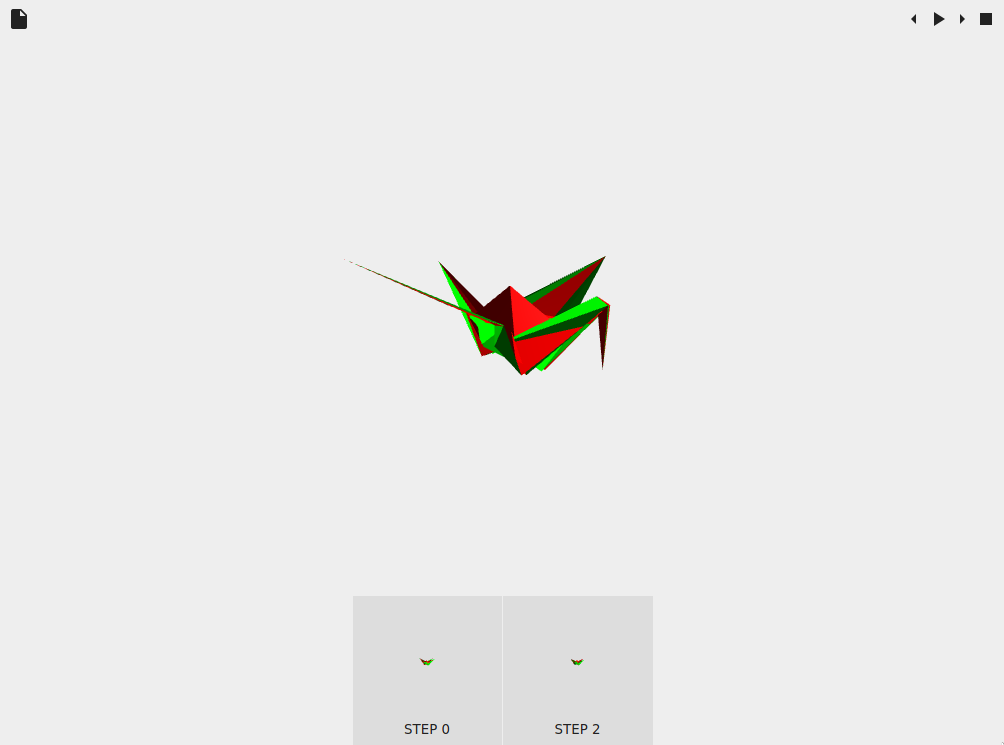
\includegraphics[width=0.8\textwidth]{assets/prototype-front.png}
\end{figure}

\subsubsection{Backend}

The current backend part is responsible for carrying out numerical computations.
It converts a provided Instruction into a set of coordinates representing
transitions between folding steps.\\

The solver is based on the techniques presented in the publication by A. Ghassaei.\cite{origami-simulator:paper}.

The computational framework consists of the three most important forces,
that drive the folding process.

\begin{description}
	\item[Beam force] - responsible for preserving edge length
	\item[Face force] - responsible for preserving the original face shape
	\item[Crease force] - responsible for folding
\end{description}

Given the current vertices' positions, and the mountain-valley assignment,
the solver computes forces imposed on vertices, and calculates their next position
using the forward Euler integration.

An additional \textbf{damping force} is introduced to prevent solver from
high frequency oscilations, assuring numerical stability under most conditions.\\

The solver is implemented in \tech{Python}, using \tech{numpy} and \tech{scipy} libraries. 


\begin{figure}[H]
	\caption{Visualization of vertices (dots), and forces applied to them (arrows)
	during folding of a rectangular sheet of paper in half, along the diagonal. }
  \centering
    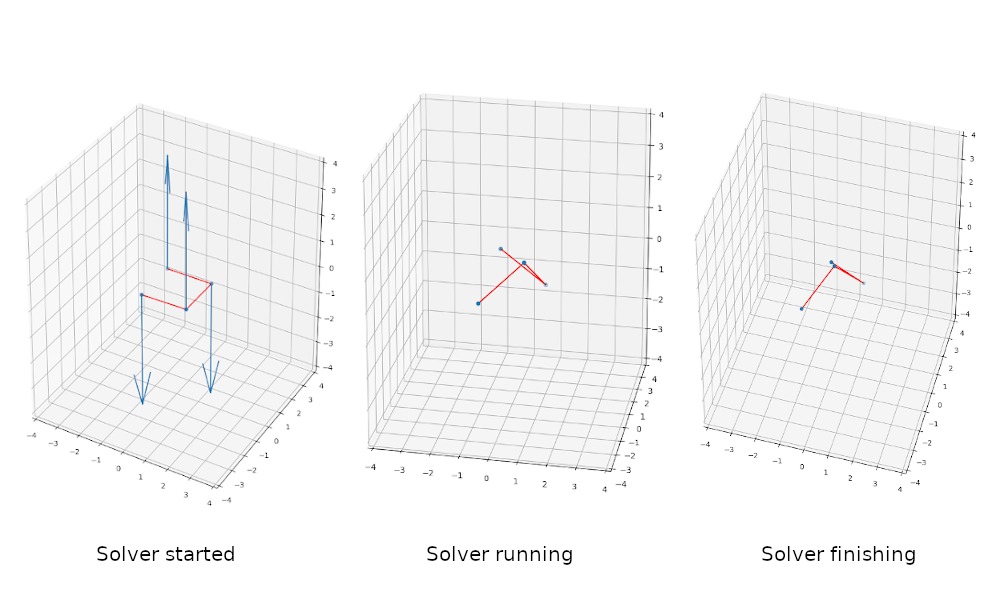
\includegraphics[width=0.8\textwidth]{assets/prototype-backend.png}
\end{figure}


\subsection{Project overview}
\label{section:project-overview}

As a name for our project, we picked \textbf{Origuide}.
We will use this code name interchangeably with terms like \textit{the system} or \textit{the application}.
\smallskip

\begin{figure}[H]
	\caption{High level system overview}
  \centering
    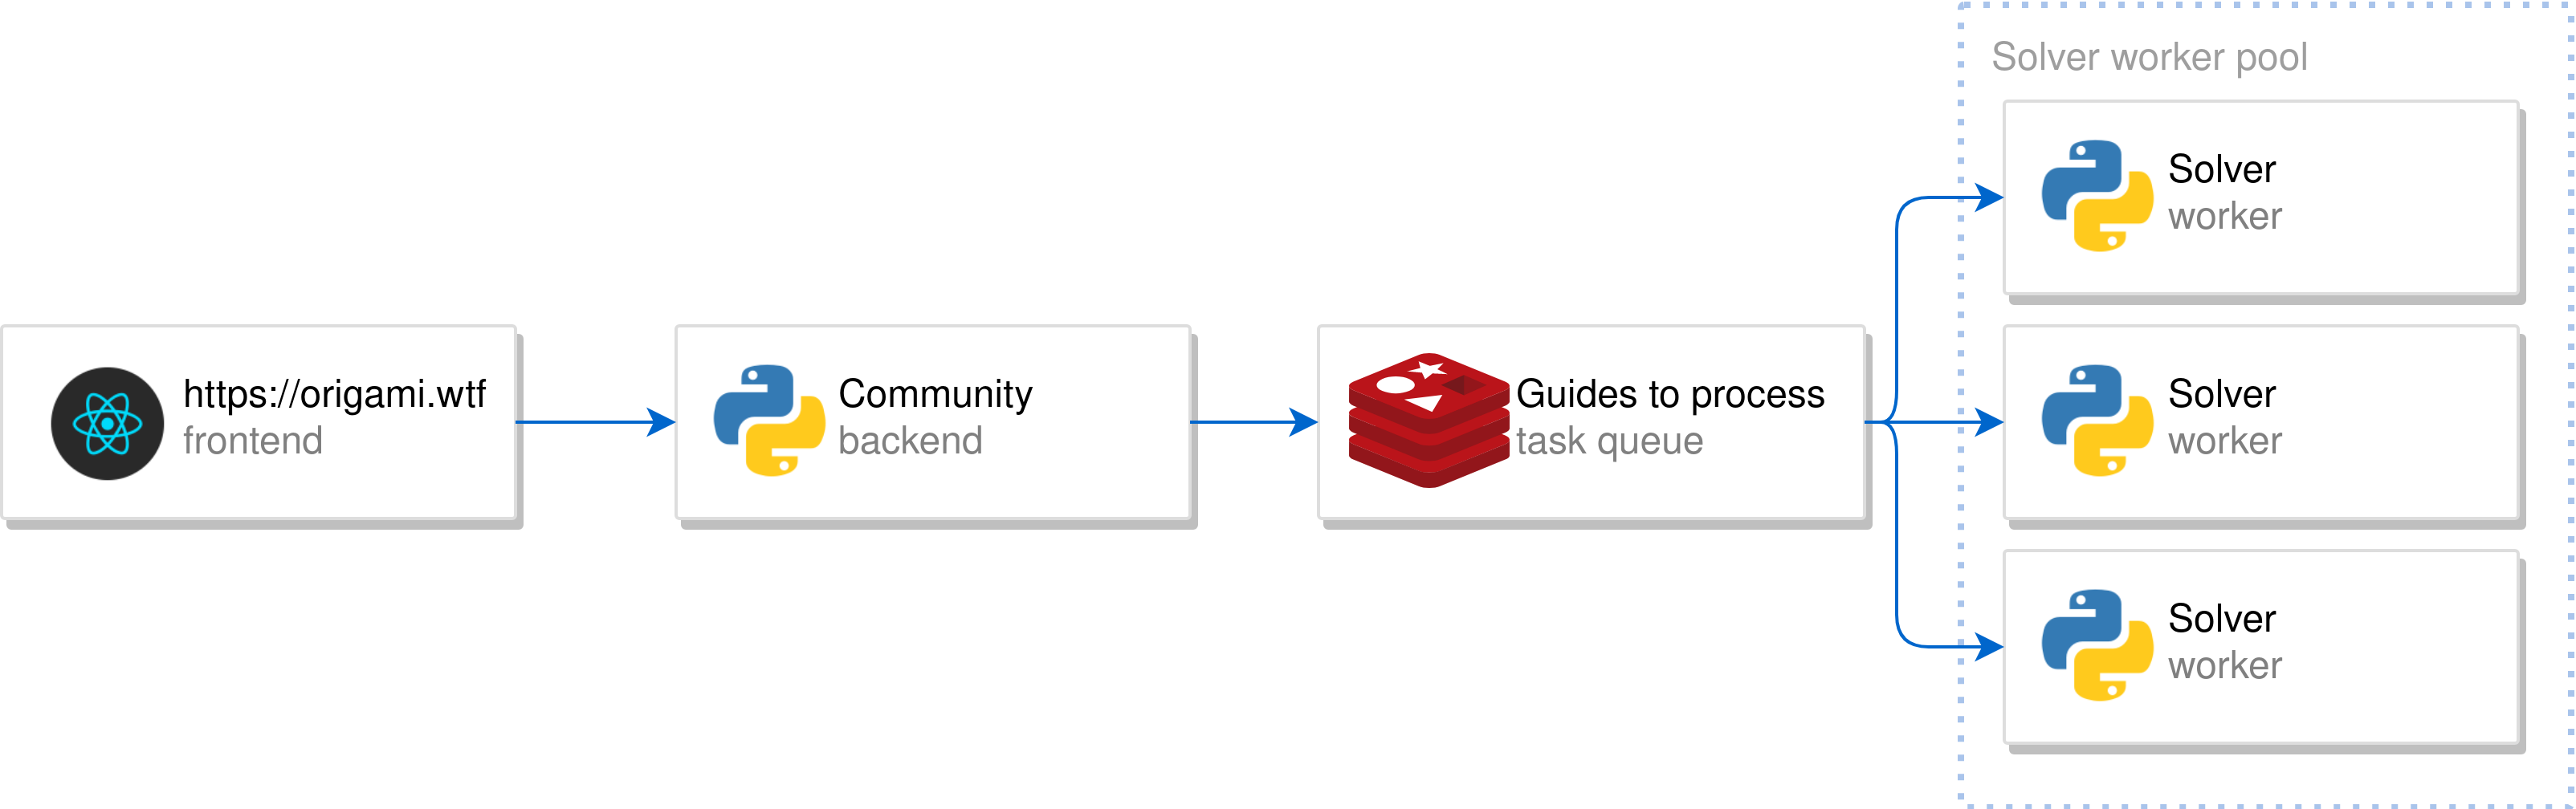
\includegraphics[width=\textwidth]{assets/architecture.png}
\end{figure}

Origuide consists of the following layers:
\begin{description}
	\item[Frontend] - a component that handles all user interactions with the system. 
	\item[Backend] - a component responsible for: \begin{itemize}
		\item processing all user requests initiated on the Frontend
		\item managing persistent data 
		\item authentication and authorization
		\item scheduling of Instruction processing
	\end{itemize}
	\item[Guides to process] - a task queue distributing guides to process among Solver workers
	\item[Solver worker] - a component responsible for converting Instructions to Guides.
\end{description}

As we previously distinguished two types of users in the system, there are two main success paths through the application.

\begin{figure}[H]
	\caption{Designer's success path}
  \centering
    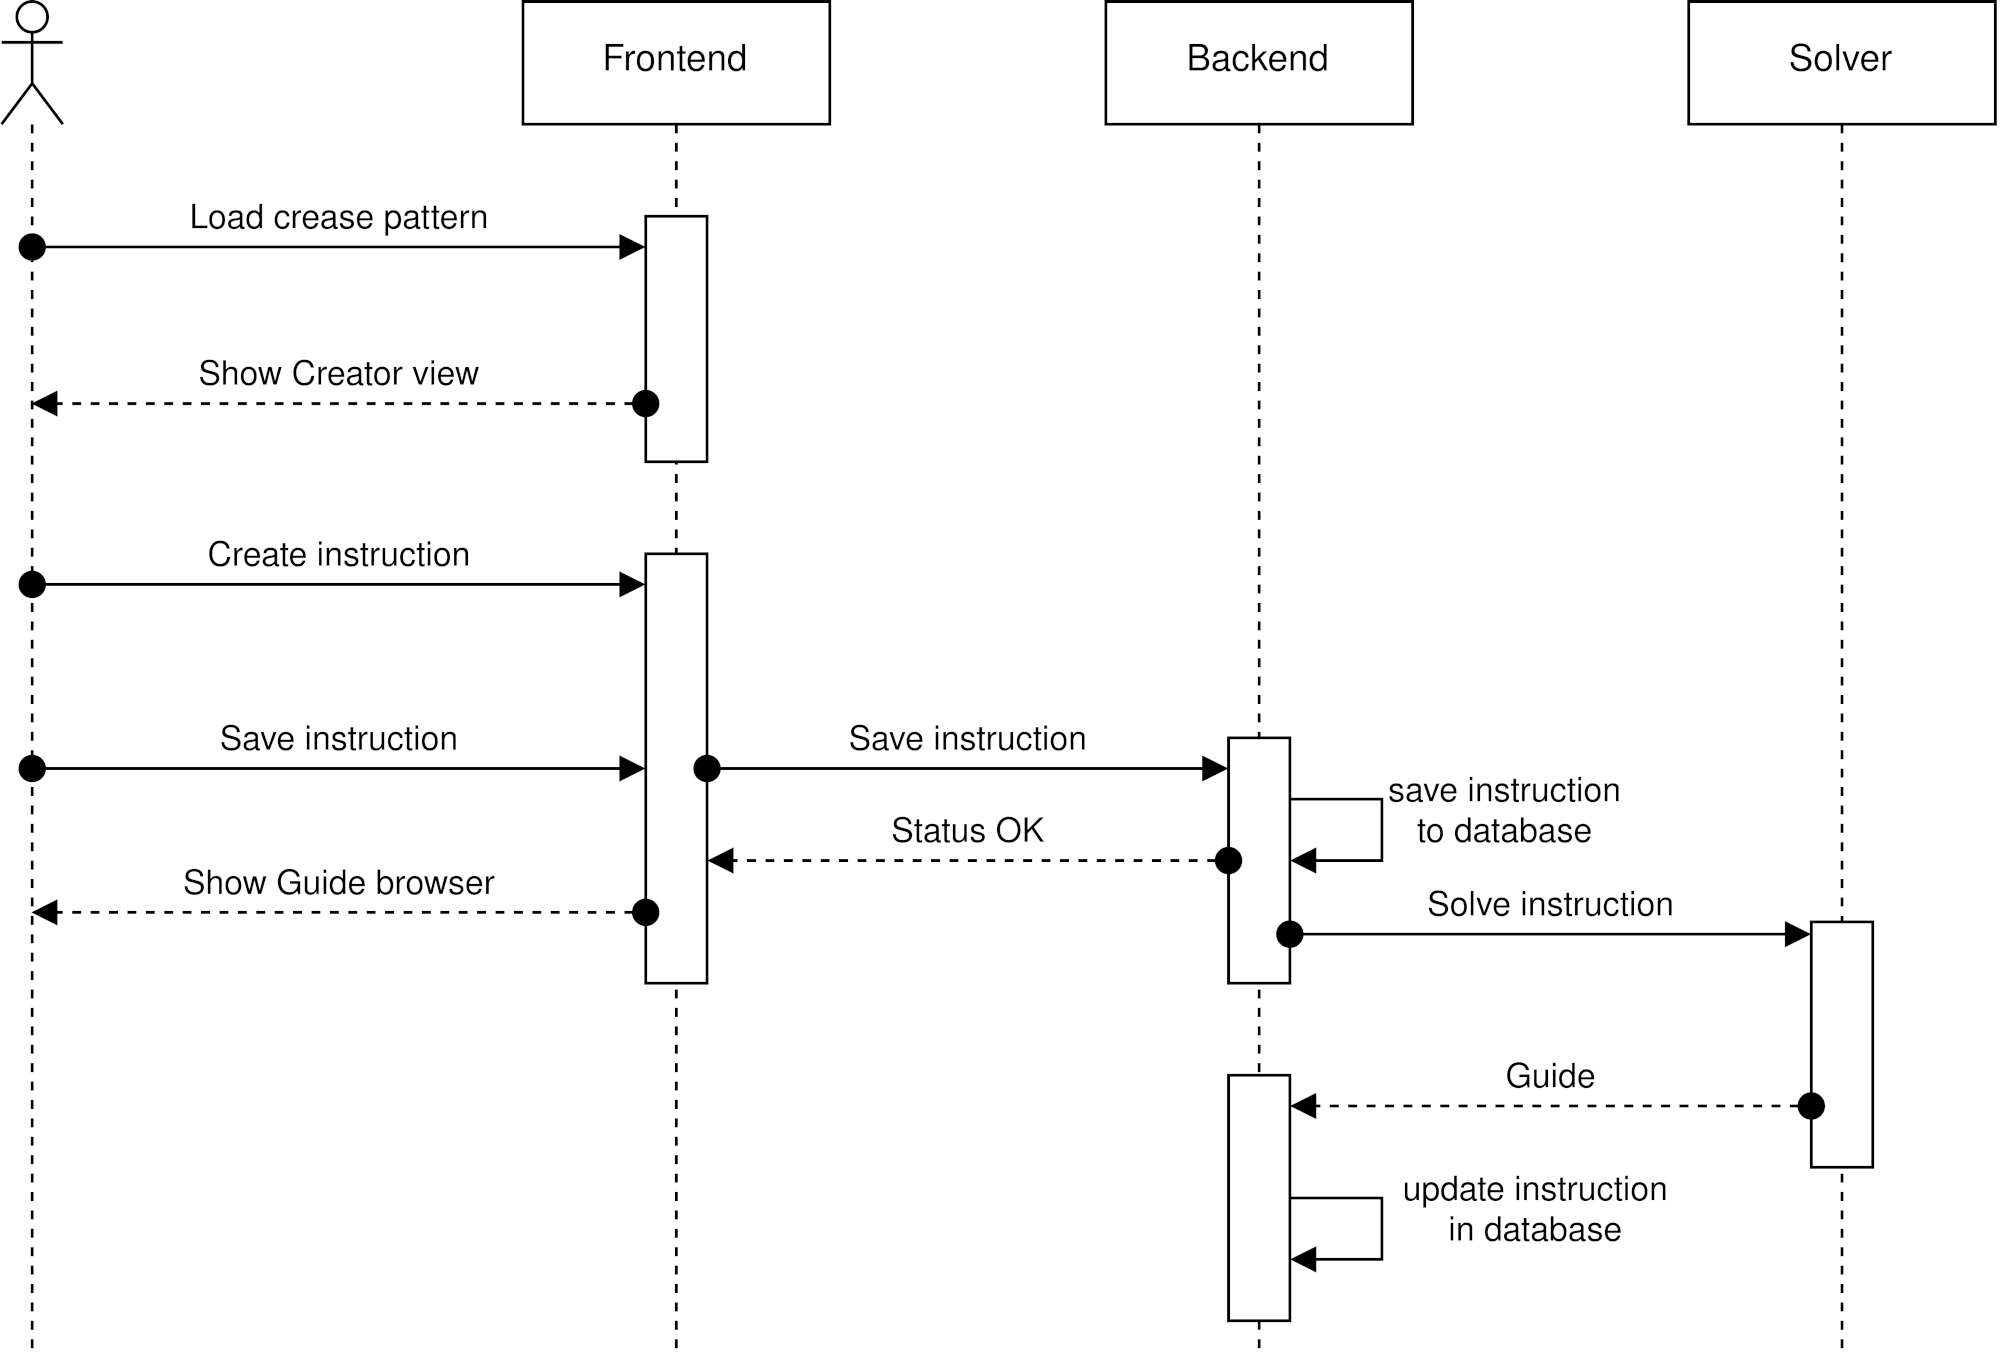
\includegraphics[width=\textwidth]{assets/3-designer-flow.png}
\end{figure}

The Designer's main objective is to create Guides. After uploading a Crease Pattern, the Designer is required to provide instruction steps. When an Instruction is saved it gets scheduled on a Task Queue and processed by a Solver worker. Once processing is finished the Guide is marked as solved in the database.

\begin{figure}[H]
	\caption{Folder's success path}
  \centering
    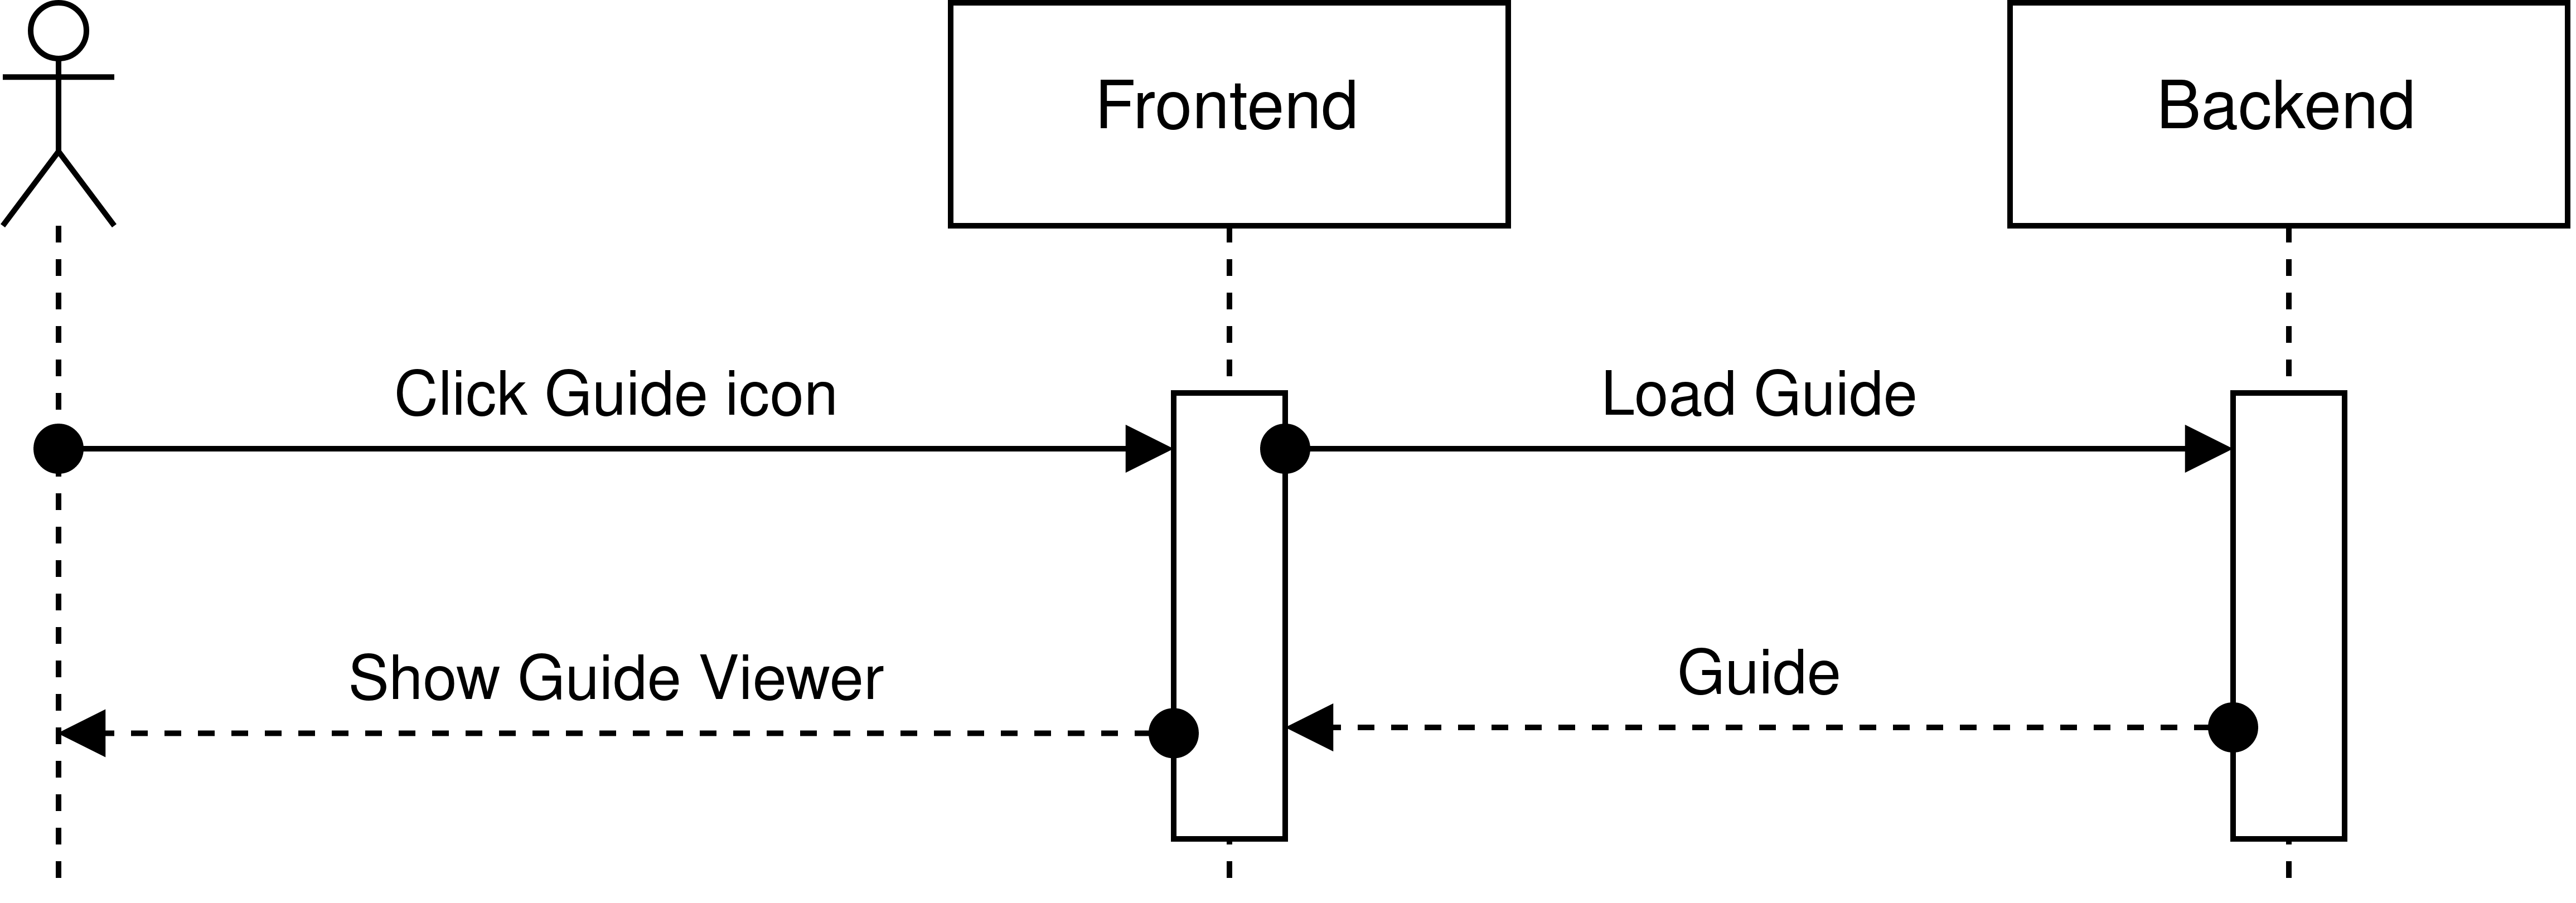
\includegraphics[width=\textwidth]{assets/3-folder-flow.png}
\end{figure}

The Folder's main objective is to fold origami figures following steps presented by the Application. After successfully retrieving a guide from the Backend, the user is presented with a Guide Viewer.

\subsection{Technology stack}

\subsubsection{Frontend}

\begin{itemize}
	\item The Application is built in \tech{Javascript} using the \tech{React} framework. 
	\item \tech{Three.JS} is used to display 3D models.
	\item Triangulation is done using \tech{earcut}. 
	\item Parsing folds is aided by \tech{fold}.
	\item User Interface components come mainly from \tech{Material-UI}.
	\item \tech{Webpack} is responsible for bundling, minimizing, and transpiling the source code.
	\item Code style is checked using \tech{Prettier} with \tech{ESLint} and enforced on every commit using \tech{Husky}.
	\item \tech{Jest} has been incorporated as a test runner.
\end{itemize}

Origuide is a web application. Hence, \tech{Javascript} has been an obvious choice. We have briefly considered \tech{Typescript} as well, but have not used it due to its more enforcing nature, which could have potentially slowed down the development process. When it comes to 3D rendering frameworks \tech{Three.js} is one of the most mature and most frequently used libraries for modern rendering targets such as \tech{WebGL}. The decision to use \tech{Material-UI} has been made without much research on other tools, which we later regretted. As previously mentioned, we have also introduced \tech{React} early in the process to aid us with state management and organize the frontend application in a structurized manner. The tools chosen for code and software quality assurance have been picked based on our familiarity with them.


\subsubsection{Backend}

\begin{itemize}
	\item Backend is built in \tech{Python} using \tech{Django} framework. 
	\item \tech{DjangoRestFramework} simplifies a REST server setup.
	\item \tech{drf-base64} helps with decoding base64 encoded files.
	\item \tech{PyJWT} assists in authentication processes.
	\item \tech{factory-boy} is used to generate testing data.
	\item Data is stored in a \tech{PostgreSQL} database.
	\item \tech{Celery} was chosen for asynchronous task processing.
	\item \tech{Redis} acts as a task queue for \tech{Celery}.
\end{itemize}

The Community backend technology stack has been chosen based on the maturity of tools, perceived speed of iteration, and our prior experience. \tech{Django} is an opinionated framework, which provides a set of sane default configuration for rapid prototyping and building of web applications. Choosing it has enabled us to focus on the main product instead of common security issues of HTTP servers, database access, schema migrations, password policies, or mail sending. The rest of the libraries used are strongly tied to the \tech{Django} community and recommendations.

\subsubsection{Solver}

\begin{itemize}
	\item Solver runs under \tech{Python}'s alternative implementation - \tech{PyPy}.
	\item \tech{Shapely} is used for triangulation.
\end{itemize}

At first, Python was meant to be used only for building a proof of concept to answer the question of whether implementing a solving library on the backend, instead of the frontend, is a feasible solution for the project. The question has been answered affirmatively, and at that moment we were quite happy with the performance aspect. Unfortunately, down the line, after loading more and more complicated Origami models it became apparent that Python's native performance will not cut it. We were worried that a whole rewrite in a more performant language is imminent. After seeking an alternative solution, the fear has been dispelled. The implementation has benefited from a ten-fold increase in performance by using a performance-oriented Python implementation - \tech{PyPy}.



\subsection{Components overview}
% Przegląd poszczególnych komponentów a wiec np. baza danych, aplikacja typu klient, serwis RESTowy. Jeśli baza to ERD z opisem, jeśli aplikacja kliencka to jakie elementy, widoki, jak się łączy i kiedy. Jeśli prosta aplikacja WWW to można pokazać strukturę projektu. Jeśli serwis RESTowy to jego specyfikacja z przykładami. Protokół komunikacji to może być zupełnie osobny opis. %

\subsubsection{Frontend}

The web application contains two main subcomponents: \textit{Guide Creator} and \textit{Guide Viewer}, responsible respectively for: creating instructions and viewing animated guides. Other pages are mainly related to the community aspect and will only be covered superficially in this section.

\begin{figure}[H]
  \caption{Overview of the frontend pages and components. Grayed out pages are related to user management.}
  \centering
    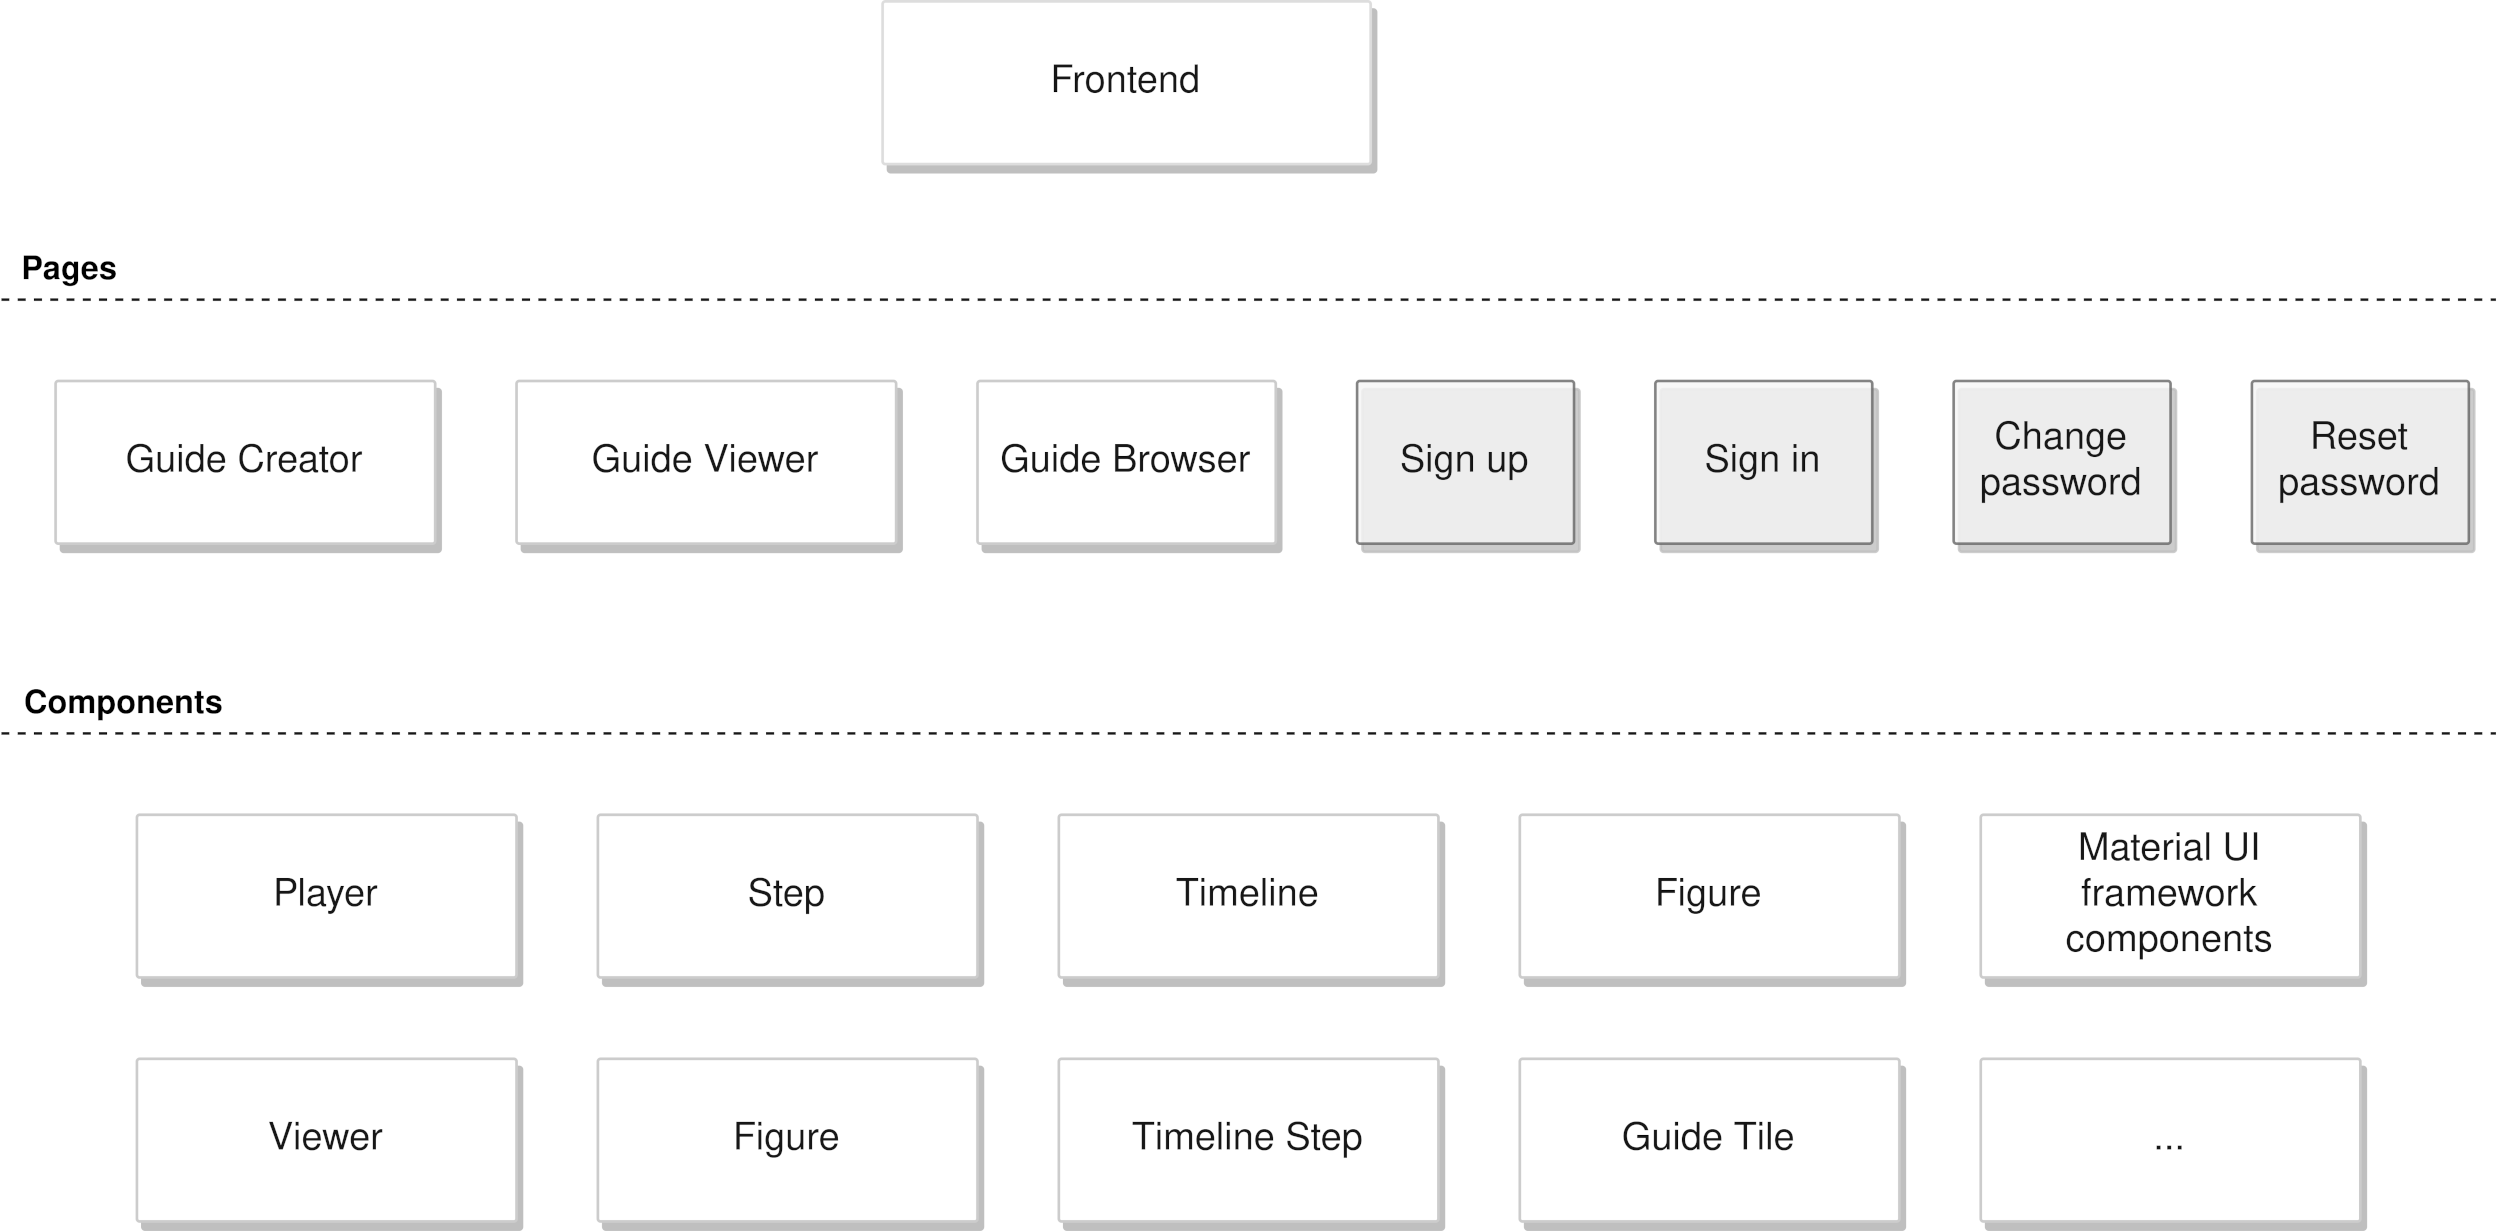
\includegraphics[width=\textwidth]{assets/3-frontend-architecture.png}
\end{figure}

The web application has been structured in a way that encourages building and reusing small components. An example would be a \textit{Viewer} component which is responsible for rendering origami figures and appears in both \textit{Guide Creator} and \textit{Guide Viewer} pages. The structure has allowed us to keep the code maintainable and implement changes quickly.

\medskip

Data storage and manipulation are powered by three stores which store data related to different aspects and functionality of the system.

\begin{itemize}
	\item The Creator store is responsible for storing an Instruction while it is being worked on.
	\item The Player store stores information about the Guide while it is being viewed.
	\item The Community store holds information regarding user sessions.
\end{itemize}

The application also contains a service responsible for communication with the Community backend.

\begin{figure}[H]
  \caption{Overview of the frontend stores and services.}
  \centering
    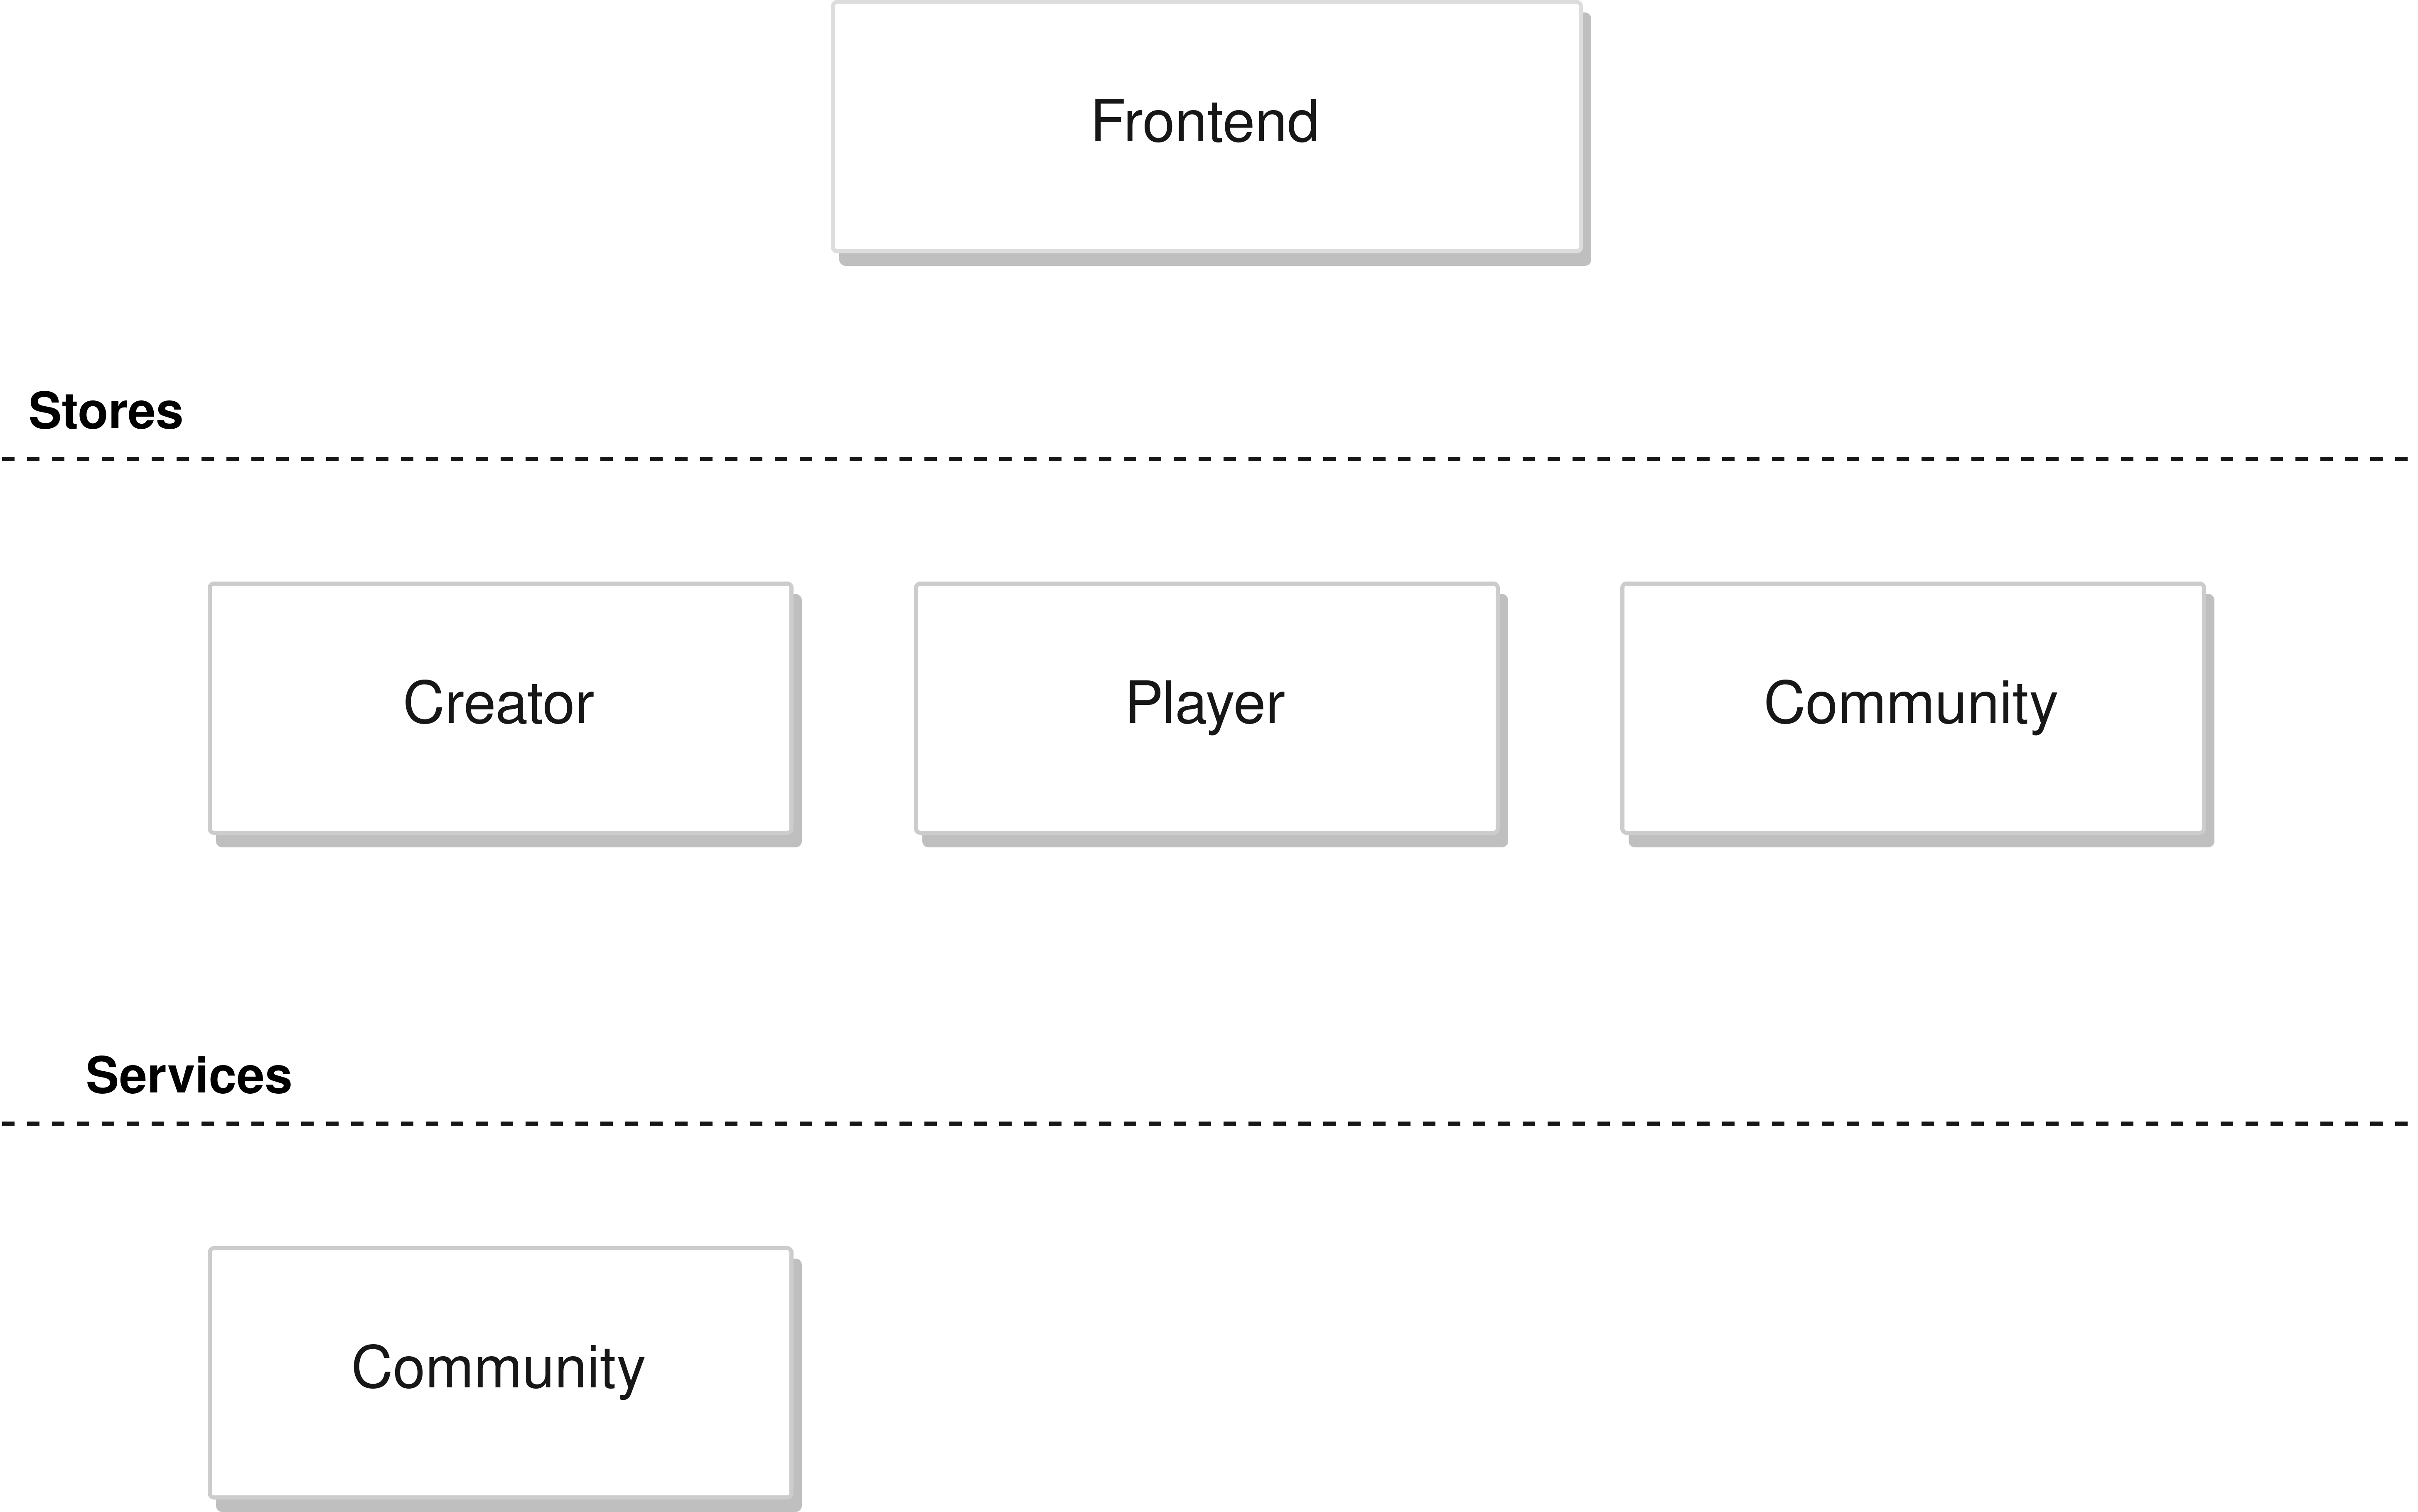
\includegraphics[width=0.7\textwidth]{assets/3-frontend-stores-services.png}
\end{figure}

\medskip


\textbf{Guide Creator}

\medskip

Guide Creator is a frontend subcomponent allowing Designers to create step-by-step Instructions from a crease pattern.


\begin{figure}[H]
  \caption{An overview of the Guide Creator}
  \centering
    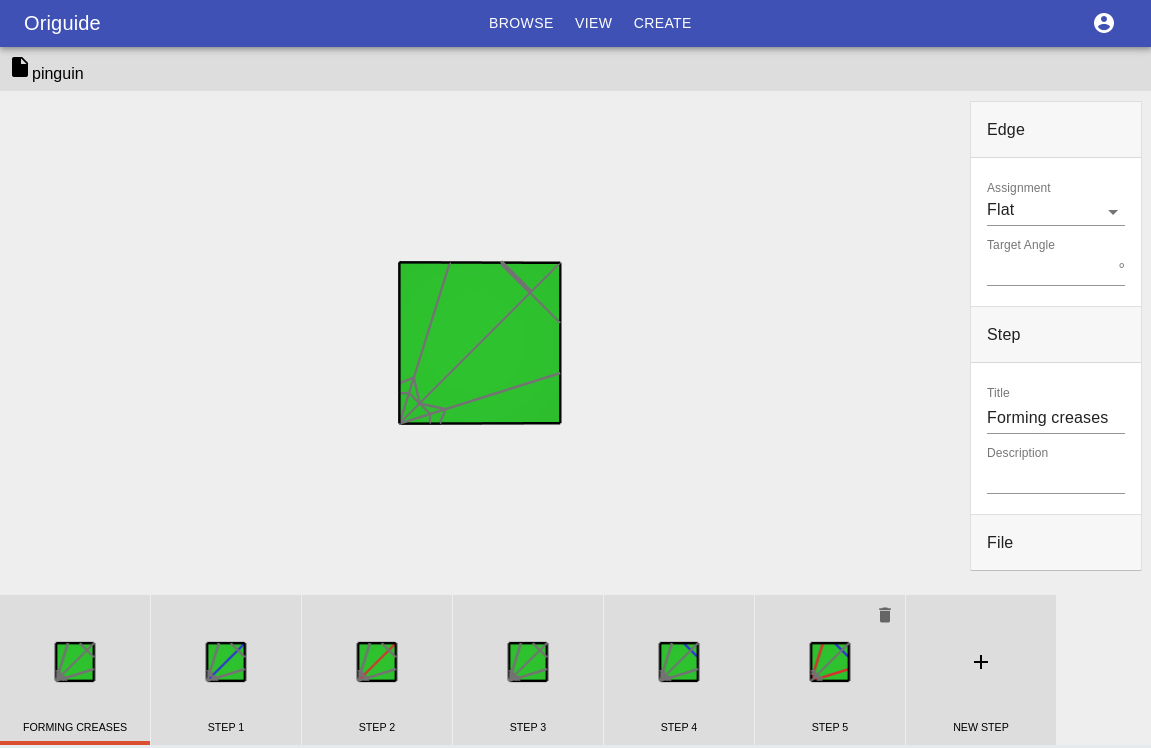
\includegraphics[width=\textwidth]{assets/3-component-creator.png}
\end{figure}

In the center one can see a loaded crease pattern with the edge assignments reflecting the currently selected step. At the bottom an interactive list of steps is shown.

\medskip

To the right there is a set of configuration sections correspondingly responsible for: \begin{description}
	\item[edge] - Setting an edge target assignment or a fixed target angle.
	\item[step] - Setting a step name and a description.
	\item[file] - Setting an Instruction name and a description.
\end{description}

\medskip

\begin{figure}[H]
  \caption{The process of creating an Instruction using the Guide Creator from a Designer's perspective.}
  \label{3-designer-creator-flow}
  \centering
    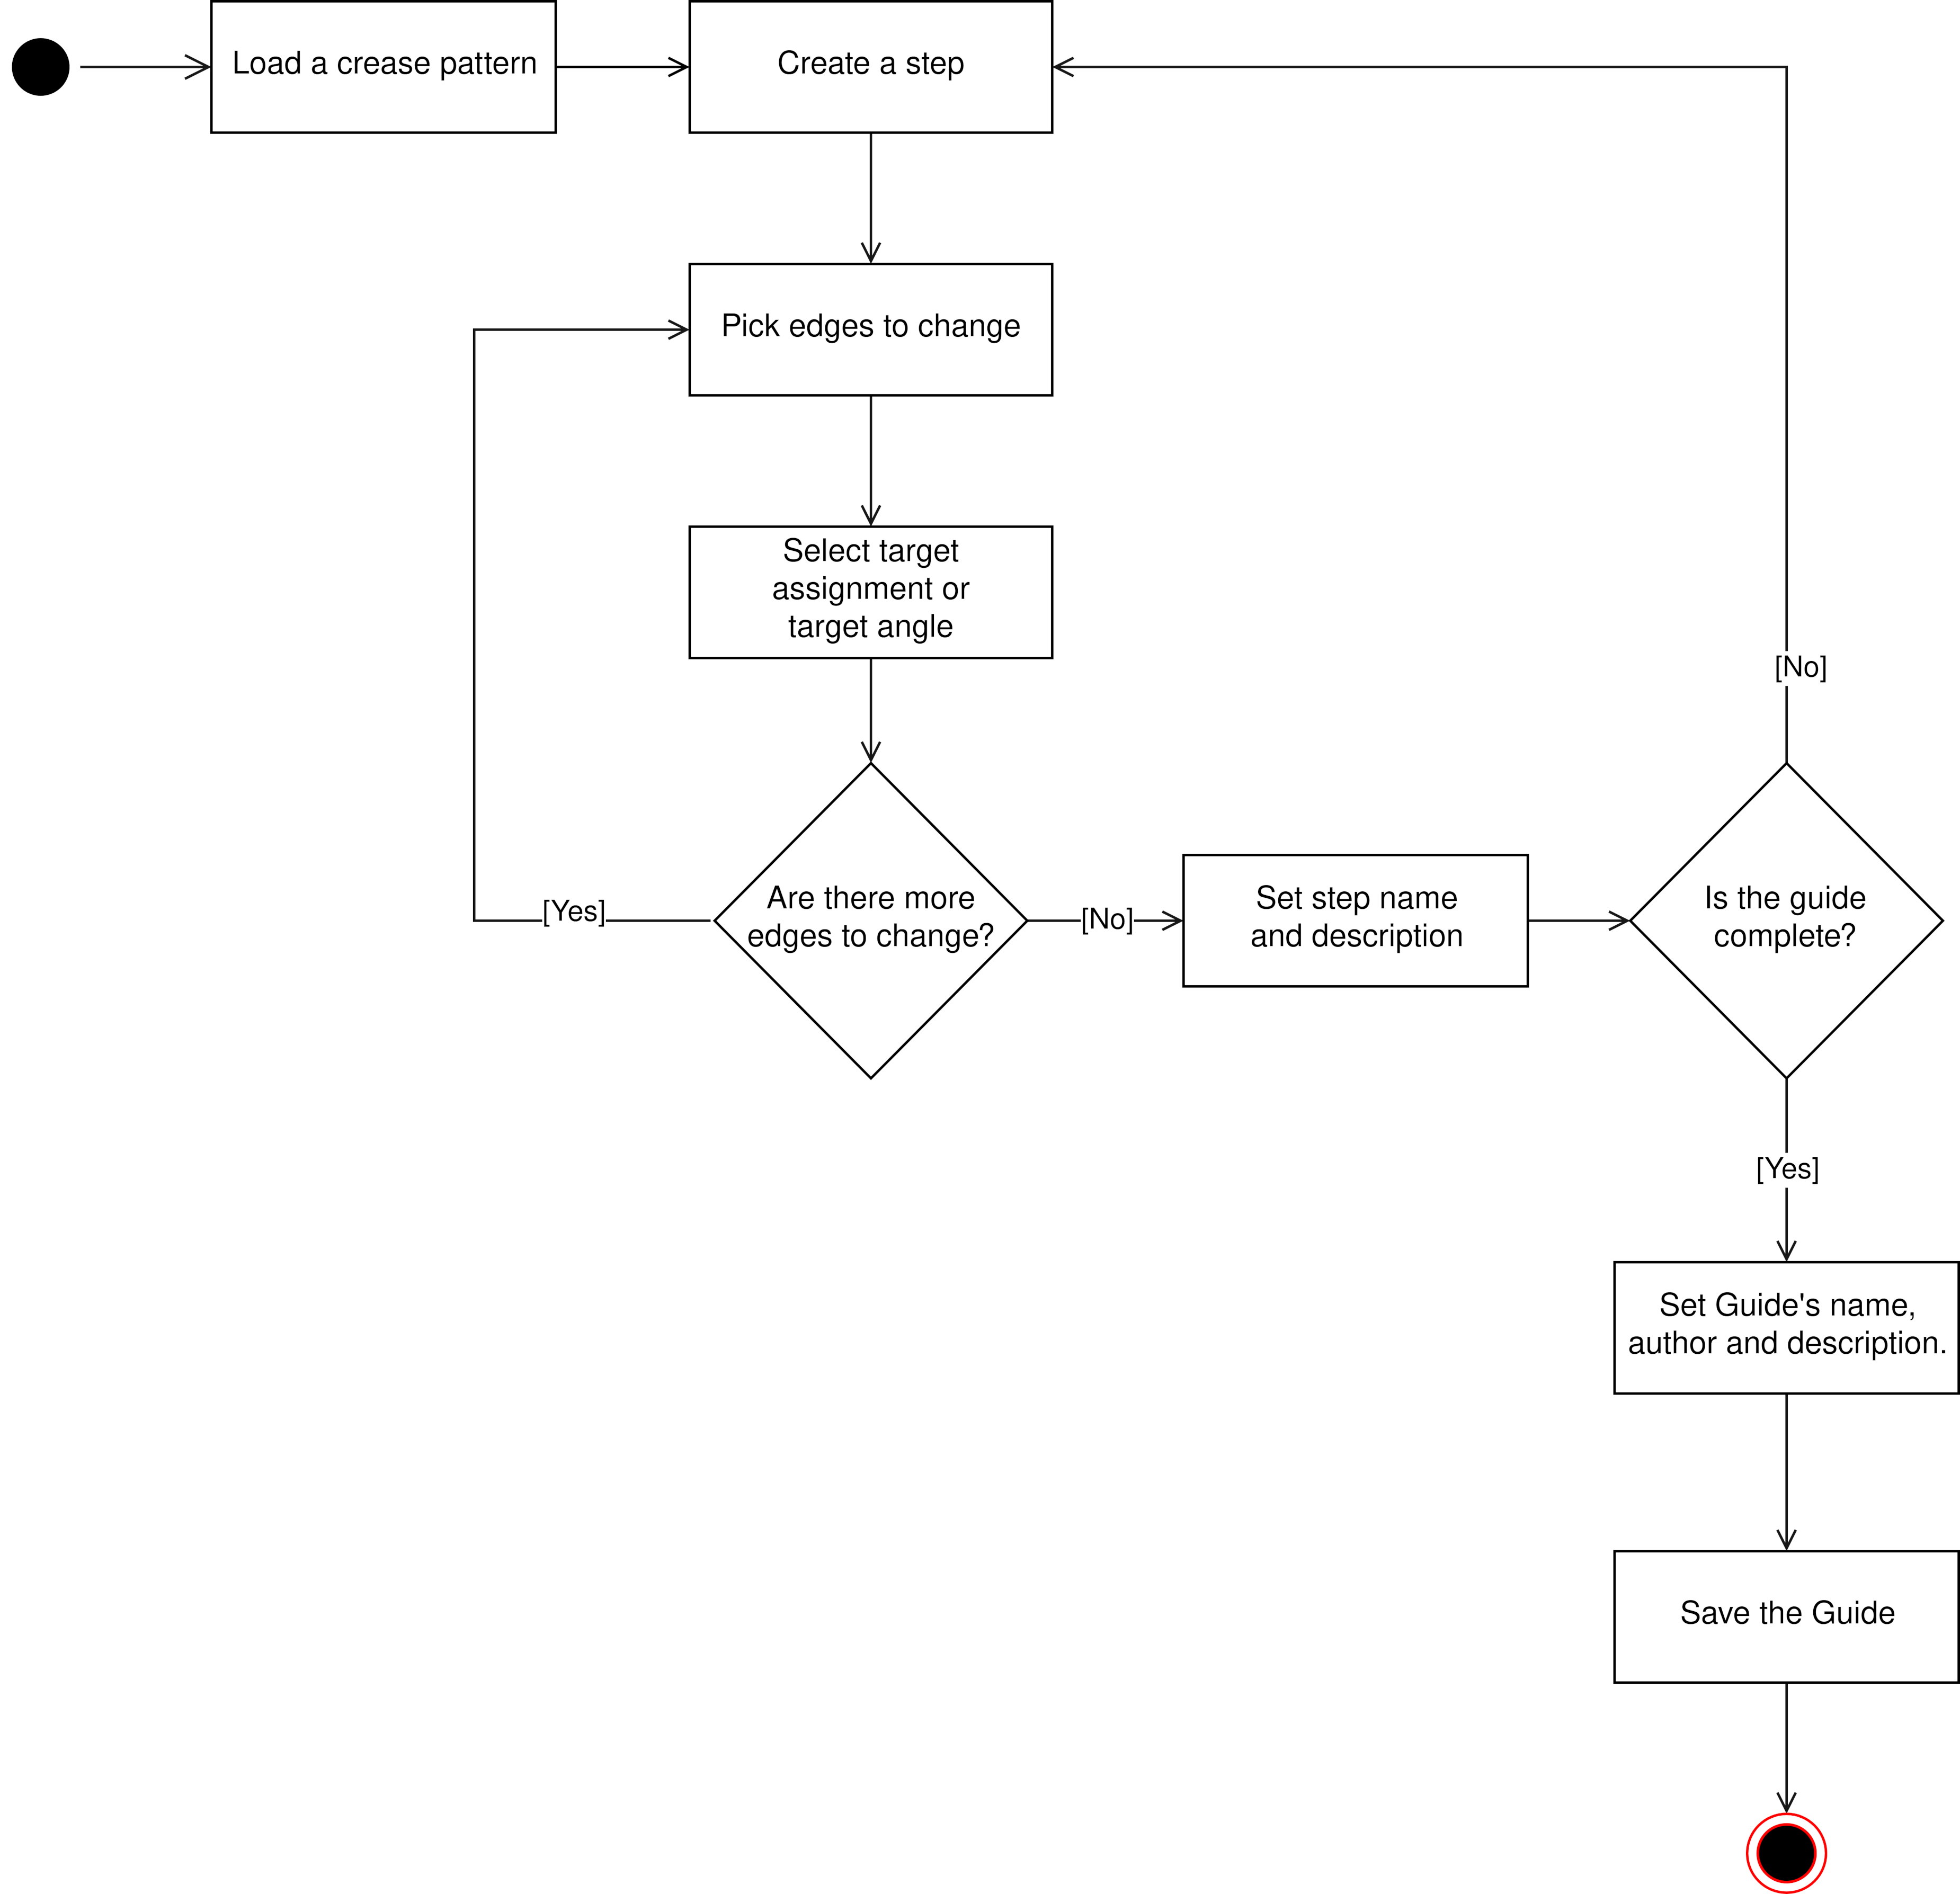
\includegraphics[width=\textwidth]{assets/3-designer-creator-flow.png}
\end{figure}

Until \textit{Save the Guide} step, all data and user actions are handled on the client-side. When \textit{Save the Guide} action is invoked:

\begin{itemize}
	\item if a user is logged in, a request is sent to the Community backend with the whole configuration attached, or
	\item a file download is initiated.
\end{itemize}

\begin{figure}[H]
	\caption{A Guide creation request. Almost all information is encoded in the \texttt{.fold} file}
	\begin{lstlisting}
{
	"private":false,
	"guide_file":"data:text/json;base64,<base64 encoded guide>",
	"thumbnail":"data:text/json;base64,<base64 thumbnail>"
}
	\end{lstlisting}
\end{figure}

\begin{figure}[H]
	\caption{A Guide creation response. The Instruction has not been processed yet, therefore, \texttt{animation\_file} is not available.}
	\label{guide-response}
	\begin{lstlisting}
{
	"id":6,
	"owner":1,
	"name":"penguin",
	"published_at":"2020-12-01T18:49:18.131223Z",
	"steps":9,
	"guide_file":"https://api.<domain>/uploads/guides/file.fold",
	"thumbnail_file":"https://api.<domain>/uploads/thumbnails/thumbnail.png",
	"animation_file":null,
	"status":"QUE",
	"private":false,
	"solved":false,
	"liked":false,
	"owner_username":"maciekmm1"
}
	\end{lstlisting}
\end{figure}


\textbf{Guide Viewer}

The purpose of the \textbf{Guide Viewer} is to show animated steps fluently. It consists of a model, a list of steps, and playback controls.

\begin{figure}[H]
  \caption{An overview of the Guide Viewer.}
  \label{3-guide-viewer}
  \centering
    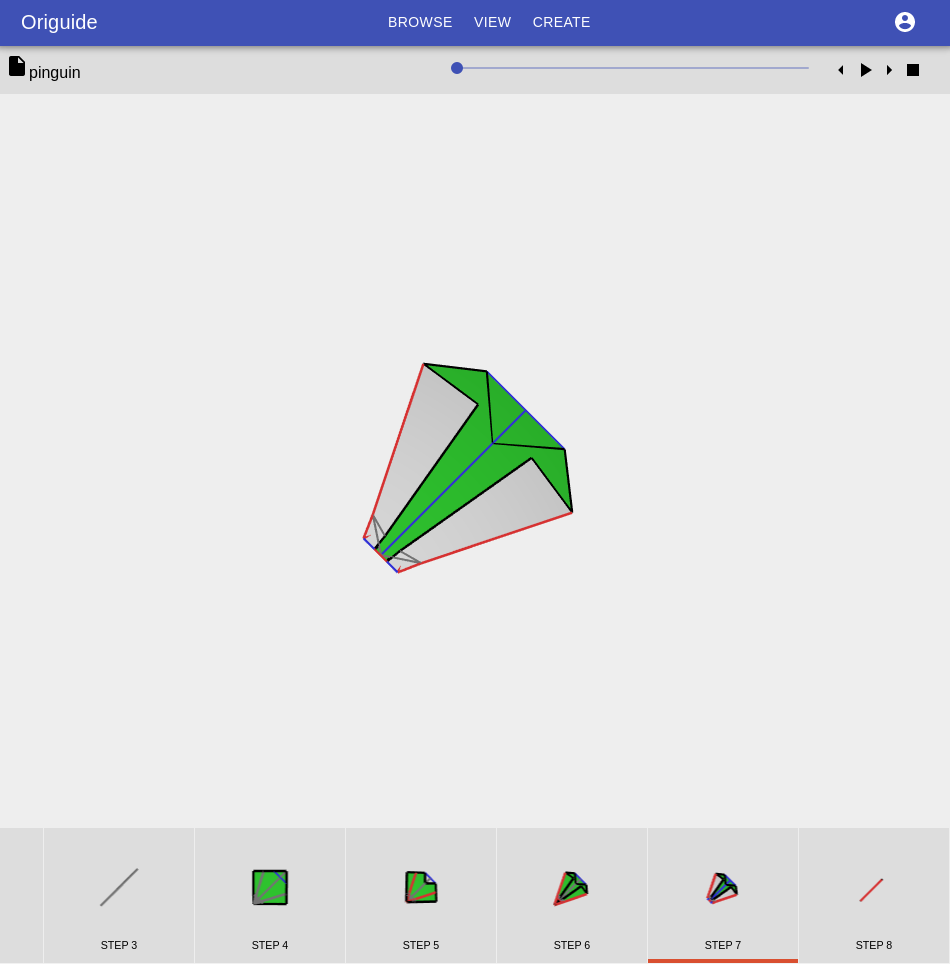
\includegraphics[width=\textwidth]{assets/3-guide-viewer.png}
\end{figure}

When a Guide is opened, the Guide Viewer fetches the \texttt{animation\_file} from the Community backend and renders it.
The response conforms to the same model as the aforementioned (\ref{guide-response}) Guide creation response.

\medskip
Playback controls allow rewinding, forwarding, stopping, and pausing. Guide Viewer also provides functionality to load an arbitrary \tech{.fold} file by clicking the file icon located in the top-left corner of the screen.


\subsubsection{Community backend}

\begin{figure}[H]
  \caption{The Community application consists of two main subapplications.}
  \label{3-backend-community-components}
  \centering
    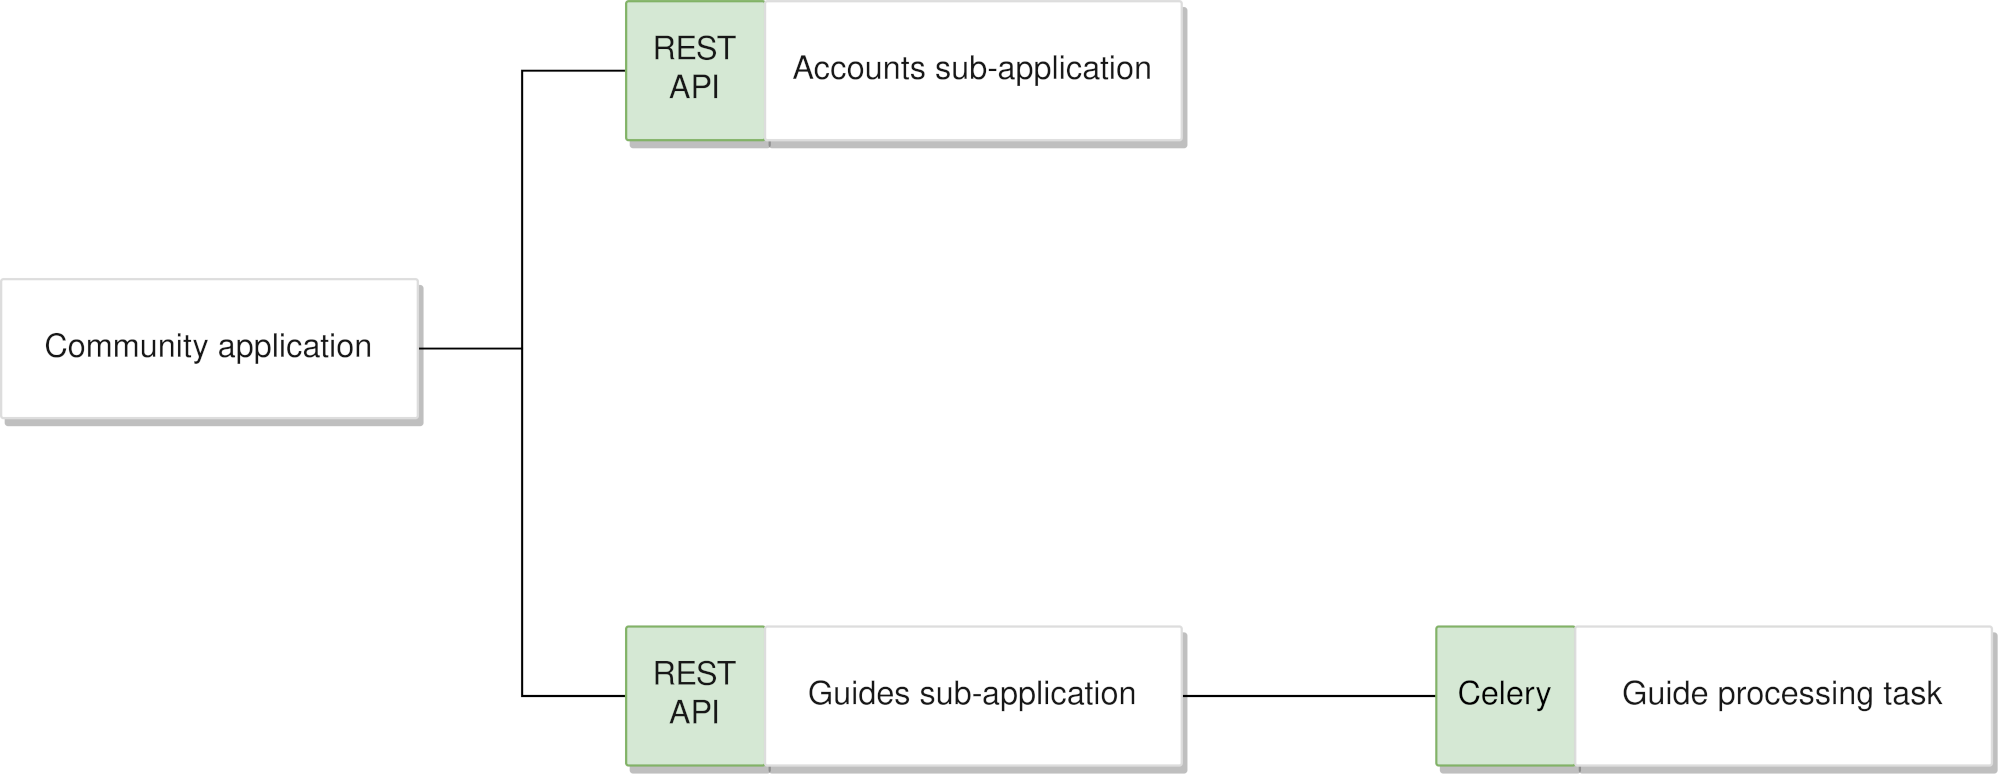
\includegraphics[width=\textwidth]{assets/3-community-application.png}
\end{figure}

The Community backend is built using \tech{Django}. It consists of a single application - Community application - that is split into a couple of subapplications:

\begin{itemize}
	\item Accounts
	\item Guides
\end{itemize}

\textbf{Guides}

Guides is the main subapplication. It is responsible for handling Guide creation, deletion, marking guides as favorites, and delegation of Guide processing tasks.

\medskip

Every action in the subapplication is performed in the context of a Guide. The figure below (\ref{model--guide}) depicts the Guide model.

\begin{figure}[H]
  \caption{ERD diagram of the model of a Guide}
  \label{model--guide}
  \centering
    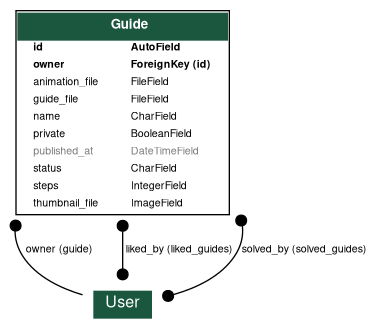
\includegraphics[width=0.6\textwidth]{assets/3-erd-guides.png}
\end{figure}

The fields describe: \begin{description}
	\item[id] - a handle for a particular Guide.
	\item[owner] - the Designer who created a particular Guide.
	\item[animation\_file] - an Animated Guide, a set of Transitions.
	\item[guide\_file] - an Instruction, a set of Steps.
	\item[name] - a name that is displayed on the website.
	\item[private] - a flag indicating whether the guide is only visible for the \texttt{owner}.
	\item[published\_at] - the date on which a Guide was published.
	\item[status] - the outcome of Instruction to Guide processing step.
	\item[steps] - a number of steps in the Guide.
	\item[thumbnail\_file] - a preview of the figure.
\end{description}

All actions initiated by a user are passed through a REST API that performs simple CRUD operations.

\bigskip

When a Guide is created or updated it is scheduled onto a task queue and later assembled into an Animated Guide. The processing task invokes Solver to calculate intermediate steps forming a smooth folding animation. 

\medskip 
Guide processing may terminate with 3 different outcomes.

\begin{itemize}
	\item An Instruction may be impossible to fold programmatically or realistically. It might occur that the solving algorithm never stops, consuming all available resources. To counteract, a hard timeout has been introduced after which the Guide is marked as timed out - \texttt{TMO}.
	\item An Instruction file may be malformed or unprocessable, in such scenario the Guide is marked as errored - \texttt{ERR}.
	\item Finally, a properly folded Instruction is marked as done - \texttt{DON}. The generated Animation file is persisted in the file system.
\end{itemize}


\begin{figure}[H]
  \caption{Guide states}
  \centering
    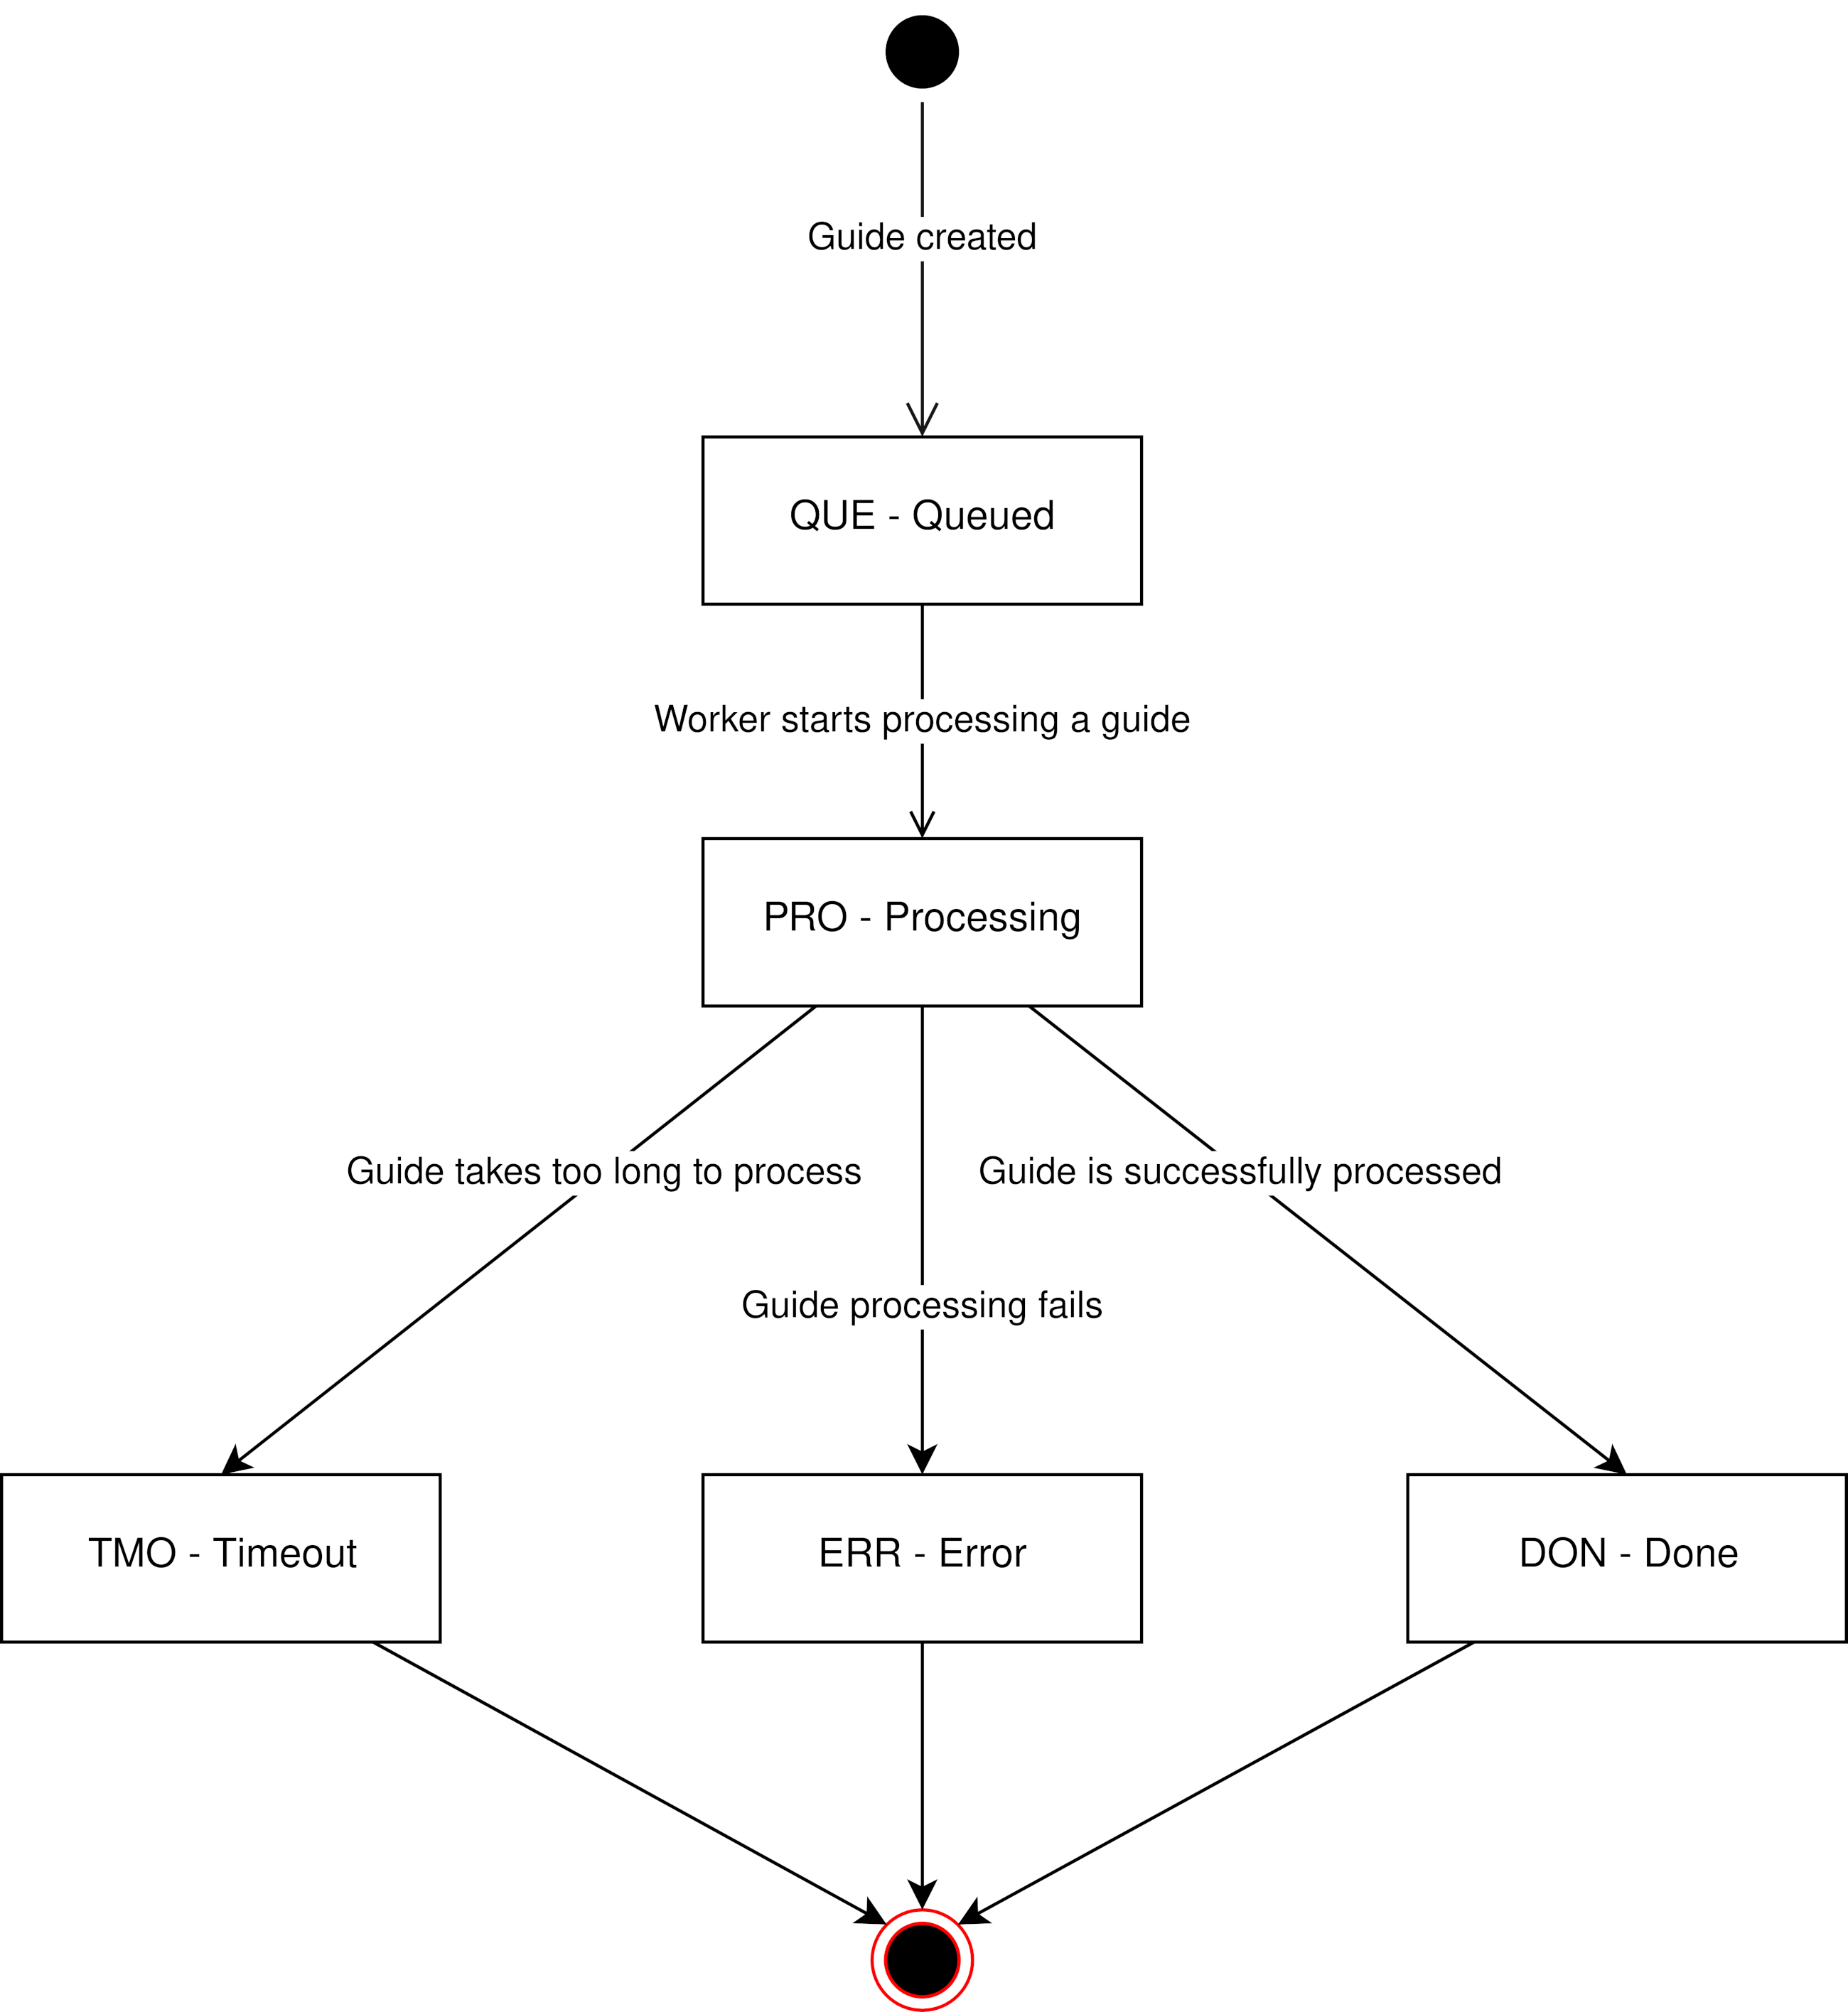
\includegraphics[width=0.8\textwidth]{assets/3-guide-states.png}
\end{figure}


\medskip

\textbf{Accounts}

Accounts subapplication's responsibilities include, but are not limited to:
\begin{itemize}
	\item authentication
	\item account creation
	\item password resetting 
	\item password changing
\end{itemize}

To fulfill its duties, the Accounts subapplication exposes several REST API endpoints.
The data model is mostly derived from the built-in Django User model, which increased the development speed considerably.
\medskip

 
\begin{figure}[H]
  \caption{Accounts - ERD diagram}
  \centering
    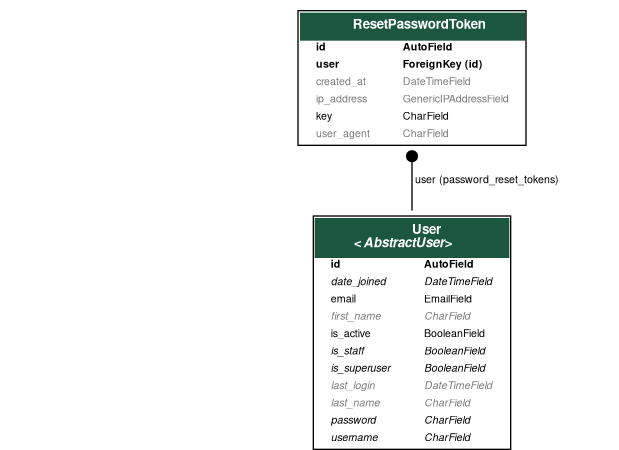
\includegraphics[width=\textwidth]{assets/3-erd-accounts.png}
\end{figure}




\subsection{Algorithms}
\subsubsection{Solver}

\textit{Please note that most of the ideas in this section come from \cite{origami-simulator:paper}}.
\smallskip

The input to the Solver is a \textit{.fold} file containing an Instruction and its output is a \textit{.fold} file containing a Guide. 
Instruction, at its simplest, is a set of vertices laying on a flat surface, and a set of edge assignments in each step.
The Solver's job is to output a resulting Guide file which has all the information necessary to display
a folding animation - that is, all the vertex positions at each step in time.

\smallskip
\textbf{Triangulation}
\smallskip

The Solver works using only triangular faces.
Therefore, before any folding-algorithm can happen, it has to generate a mesh that only consists of triangles.
\begin{figure}[H]
    \centering
    \subfloat[\centering Crease pattern before triangulation]{{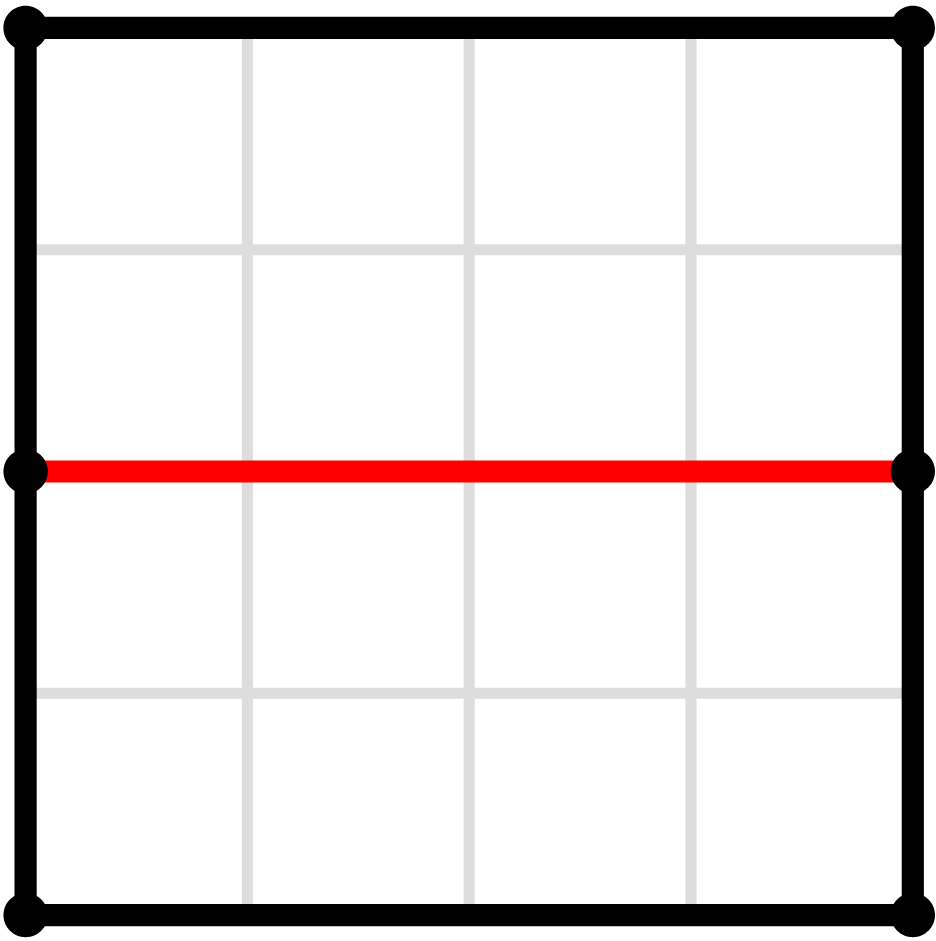
\includegraphics[width=.4\linewidth]{assets/3-2d-cp.png} }}
    \qquad
    \subfloat[\centering Crease pattern after triangulation]{{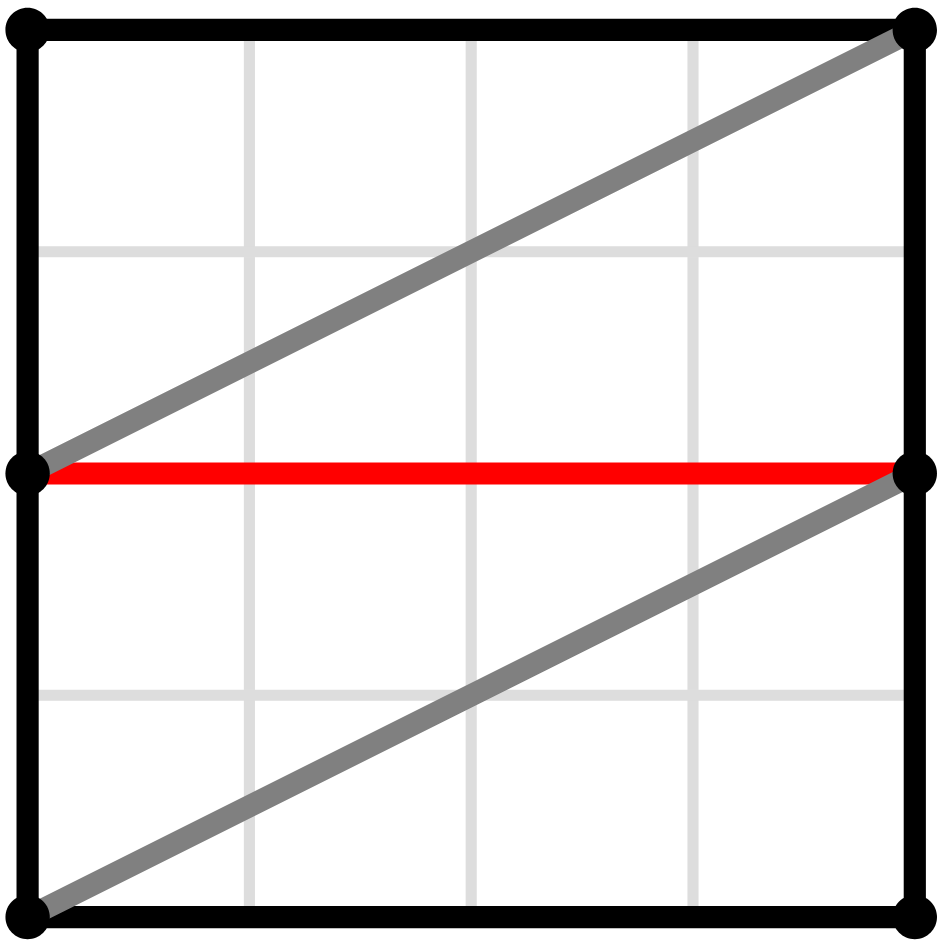
\includegraphics[width=.4\linewidth]{assets/3-2d-cp-triangulated.png} }}
\end{figure}

As an input, we get a set of 3D points, but triangulation works only in 2D.
Hence, at first we convert a set of 3D points to 2D by removing one of the axes (the one which will not lead to degenerate faces if possible).
Then, 2D \textbf{Delaunay triangulation} is carried out (we used \textit{Shapely} library for that).
The algorithm introduces new edges. These edges are dynamically constrained to stay flat while folding.

There are cases, where the default triangulation will not be satisfactory
since we would like to preserve faces' concavity and the algorithm always generates a convex polygon.

\begin{figure}[H]
	\caption{An example where triangulating a polygon marked with blue will result in an excessive triangle.}
	\centering
	\subfloat{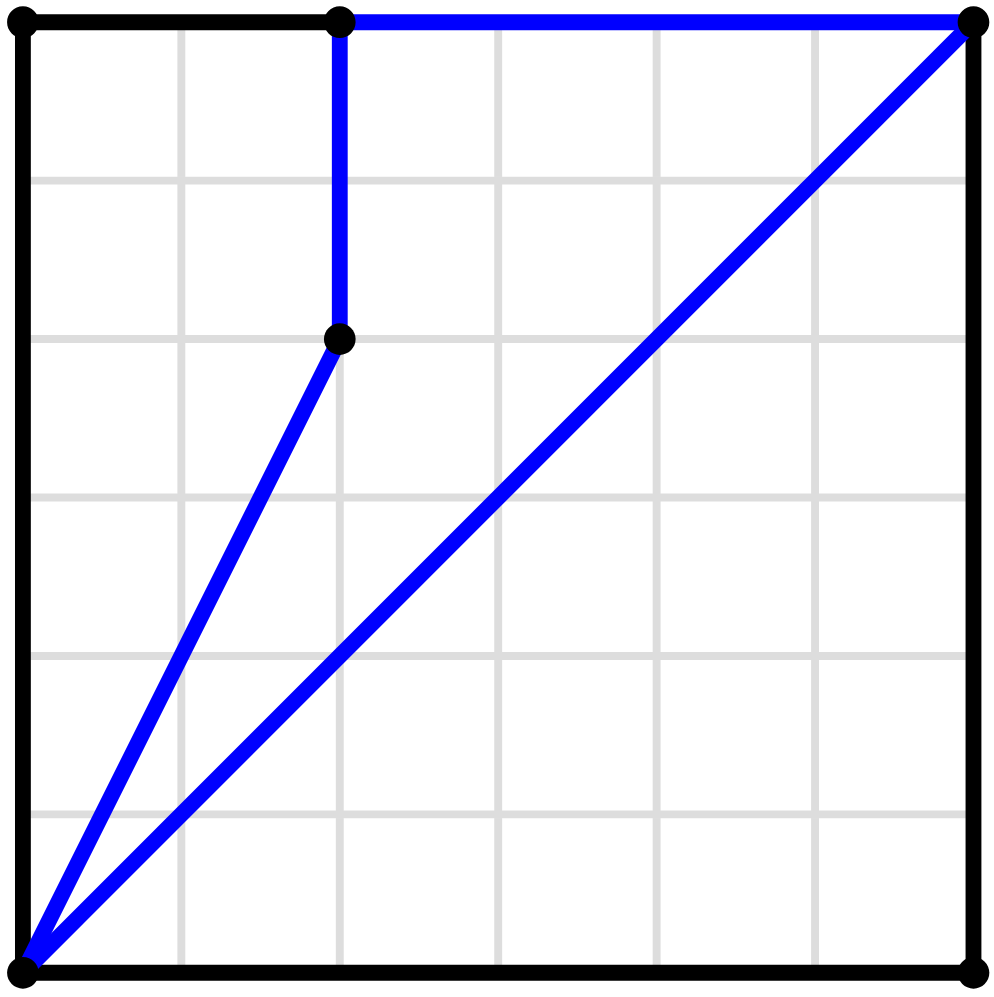
\includegraphics[width=0.5\textwidth]{assets/3-triangulation-improper-cp.png}}\qquad\qquad\qquad
	\subfloat[\centering Wrong (convex) triangulation]{{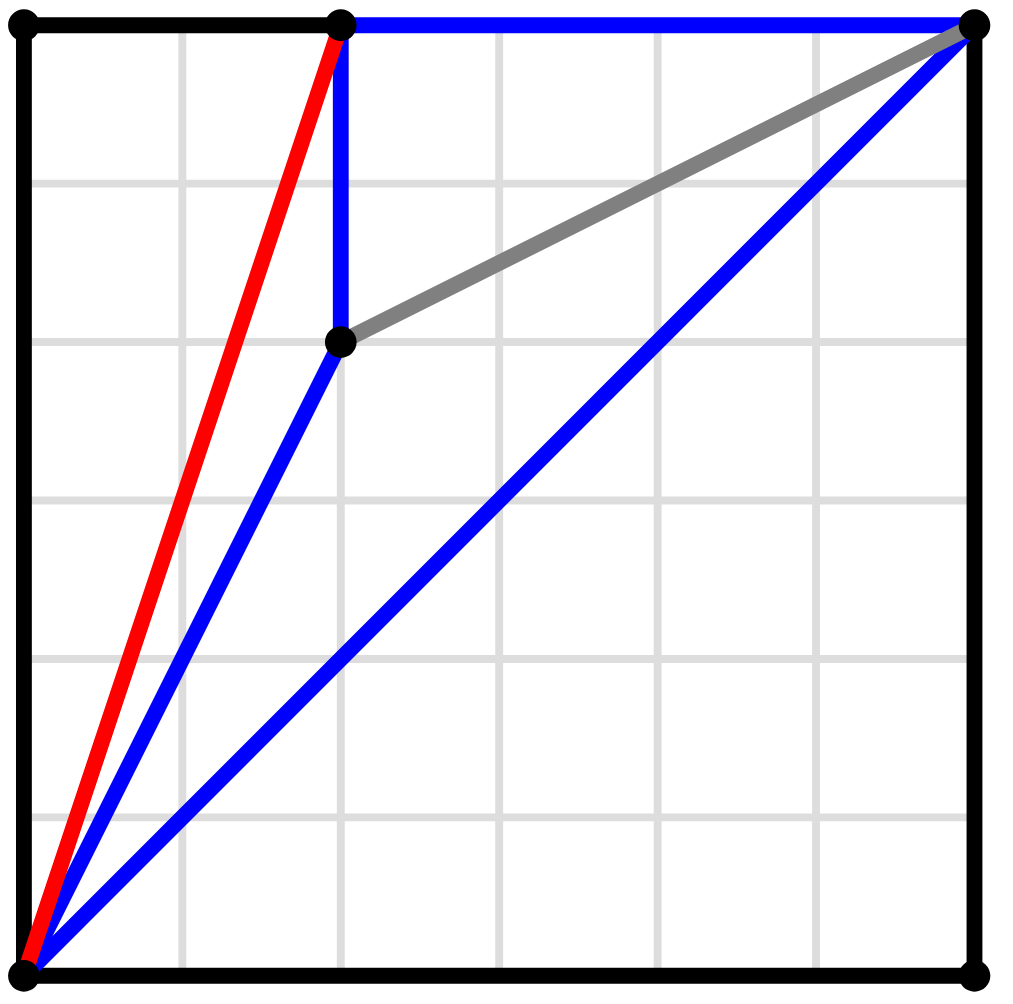
\includegraphics[width=.4\linewidth]{assets/3-triangulation-improper-cp-wrong.png} }}\qquad
	\subfloat[\centering Correct (concave) triangulation]{{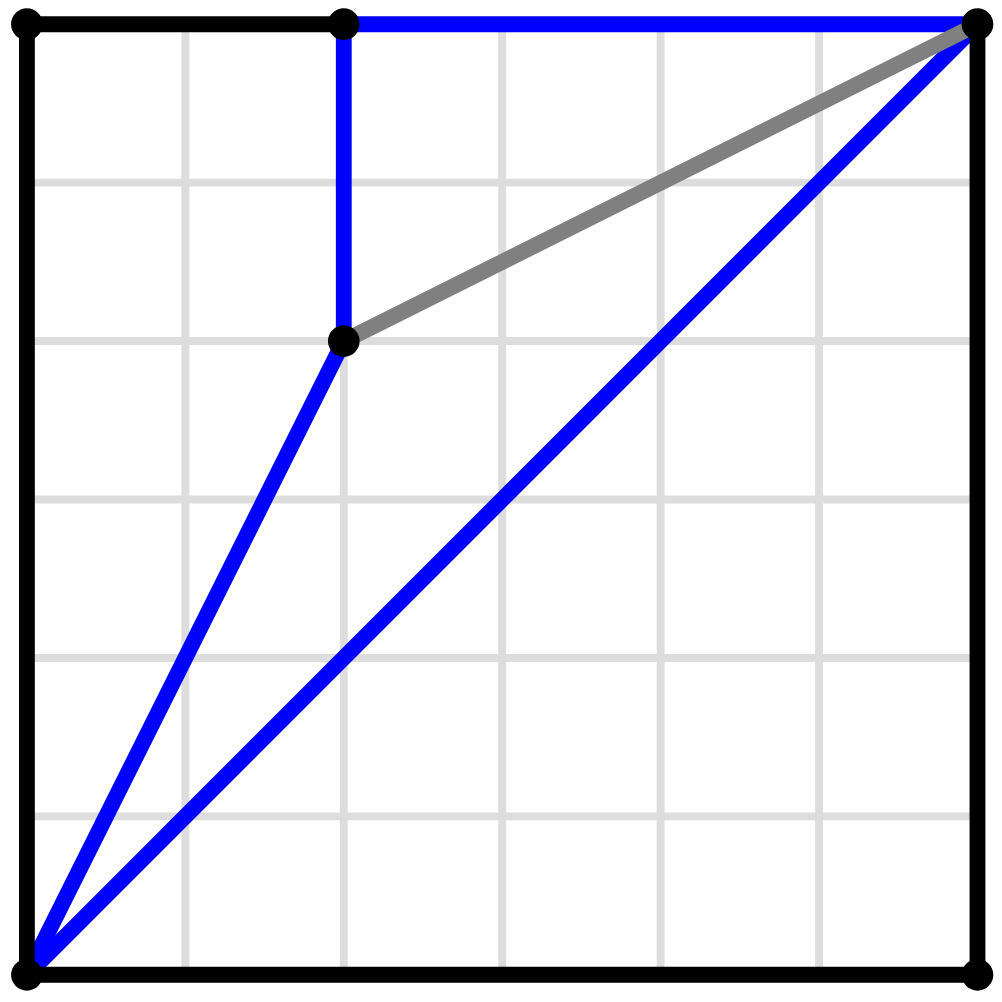
\includegraphics[width=.4\linewidth]{assets/3-triangulation-improper-cp-right.png} }}
\end{figure}

For such cases, we first compute a face's original hull. After the triangulation we check whether the resulting triangles
lay within the original hull. If they do not, they are excluded from the triangulation result.

\smallskip
\textbf{Axial constraints - beam force}
\smallskip

Axial constraints prevent stretching and compression of edges. 
Each edge is modeled as a spring which length should be kept constant at each iteration.

\begin{figure}[H]
	\caption{Visualization of edge modeling}
    \centering
	\subfloat[\centering Edge modeled as a spring]{{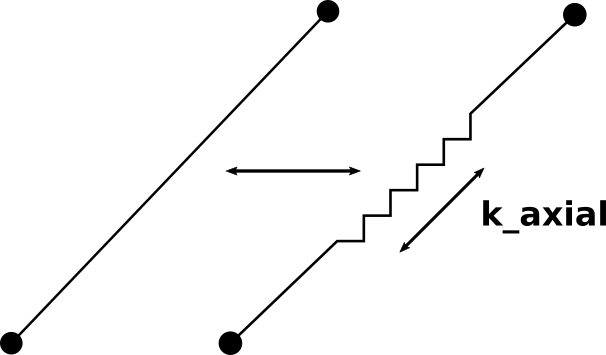
\includegraphics[width=.4\linewidth]{assets/3-edge_as_spring.png} }}
    \qquad
	\subfloat[\centering Axial constraints visualized ]{{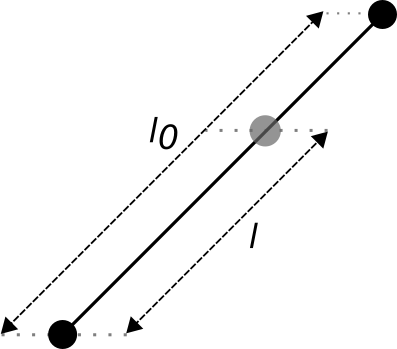
\includegraphics[width=.26\linewidth]{assets/3-edge_as_spring_l0_l.png} }}
\end{figure}

Before solving begins, the initial edge length $l_{0}$ is calculated.
Then, \textbf{Hooke's law} is used to calculate the beam force:

$$F_{l} = -k_{axial} * (l - l_{0})$$

where $l$ is the current edge length and $k_{axial}$ is a constant.

\smallskip
Before we apply the force to the vertices, first we need to convert it to a vector $\pmb{F}_{beam}$ in a model's coordinate space.
The $\pmb{F}_{beam}$ is related to the vertices position $\pmb{p}$ by:

$$\pmb{F}_{beam} = -\nabla V(\pmb{p}) = -\frac{\partial V}{\partial \pmb{p}}$$

where V is the potential energy of the system. By the chain rule, we get:

\begin{equation} \label{solver:beam_force}
\pmb{F}_{beam} = -\frac{\partial V}{\partial l}\frac{\partial l}{\partial \pmb{p}} = F_{l}\frac{\partial l}{\partial \pmb{p}} = -k_{axial} * (l - l_{0})\frac{\partial l}{\partial \pmb{p}}
\end{equation}


For the two vertices attached to the edge, we have:

$$ \frac{\partial l}{\partial \pmb{p_{1}}} = -\uveci_{12}, \frac{\partial l}{\partial \pmb{p_{2}}} = \uveci_{12} $$

where
\begin{itemize}
	\item $\uveci_{12}$ is a unit vector from vertex 1 to vertex 2
	\item $\pmb{p_{1}}$ is vertex 1 position
	\item $\pmb{p_{2}}$ is vertex 2 position
\end{itemize}

Although axial stiffness $k_{axial}$ could be related to material properties, we devised it experimentally.

All of this boils down to a few lines of code:

\lstinputlisting[language=Python]{assets/listings/beam_force.py}


\medskip
\textbf{Crease constraints - crease force}

With axial constraints we restrict the model to retain its shape while folding.
However, the main force that drives folding process is the result of crease constraints.
\smallskip

We drive faces connected by an edge to fold towards some target fold angle $\theta$.
The angle $\theta$ is the supplement of the dihedral angle between the two neighbouring triangular faces.

\begin{figure}[H]
	\caption{Crease constraints formulation between the two neighbouring triangular faces}
    \centering
	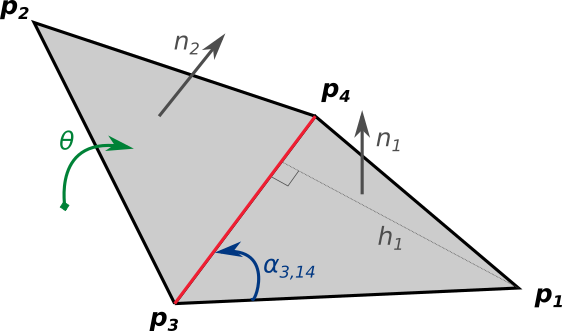
\includegraphics[width=.6\linewidth]{assets/3-crease_force_face.png}
	\label{solver:crease_force_face}
\end{figure}

Crease constraints are modeled as linear-elastic torsional springs.
Therefore, similarly to equation \eqref{solver:beam_force}, crease constraints will apply forces to the neighbouring
vertices by:

\begin{equation} \label{solver:crease_force}
	\pmb{F}_{crease} = -k_{crease}(\theta - \theta _{target})\frac{\partial \theta}{\partial \pmb{p}}
\end{equation}

where:

\begin{itemize}
	\item $\pmb{F}_{crease}$ is a force applied to a vertex in a model's coordinate space
	\item $k_{crease}$ is an edge folding stiffness (more on that below)
	\item $\theta$ is the current angle between the two faces (strictly speaking, supplement of the dihedral angle between the faces)
	\item $\theta _{target}$ is the desired angle between the two faces
\end{itemize}

In the implementation, there are 5 possible edge assignments:

\begin{enumerate}
	\item valley
	\item mountain
	\item flat
	\item boundary
	\item unknown
\end{enumerate}

$k_{crease}$ depends on the edge type.

The following piece of code computes the correct $k_{crease}$:

\lstinputlisting[language=Python]{assets/listings/crease_force_edge_assignment.py}

Let's introduce symbols:
\begin{itemize}
	\item $k_{fold} =$ \lstinline{CONFIG['FOLD_STIFFNESS']}
	\item $k_{facet} = $ \lstinline{CONFIG['FACET_STIFFNESS']}
\end{itemize}

As one can notice, the stiffness will be proportional to the initial edge length.
The stiffness parameter is chosen so that $k_{axial} \gg k_{fold}$.

Manipulating $k_{facet}$ influences how the material behaves. The smaller it is the more it acts like a piece of fabric.
The bigger it gets the more it starts to resemble paper and then plastic or metal.
\smallskip

As well as $k_{crease}$, angle $\theta _{target}$ also depends on the edge type:

$$
\theta _{target} =
\begin{cases}
	< 0 & \quad \text{for a mountain crease}\\
	> 0 & \quad \text{for a valley crease}\\
	0 & \quad \text{otherwise}
\end{cases}
$$

By default, the target angle will be one of: $\pi, -\pi, 0$, but the provided Instruction can override the default target angle.
\smallskip

Finally, partial derivatives of $\theta$ with respect to $\pmb{p}$ are given by:

\begin{equation} \label{solver:crease_force1}
\frac{\partial \theta}{\partial \pmb{p}_1} = \frac{\pmb{n}_1}{h_1}
\end{equation}

\begin{equation} \label{solver:crease_force2}
\frac{\partial \theta}{\partial \pmb{p}_2} = \frac{\pmb{n}_2}{h_2}
\end{equation}

\begin{equation} \label{solver:crease_force3}
	\frac{\partial \theta}{\partial \pmb{p}_3} = \frac{-\cot{\alpha _{4,31}}}{\cot{\alpha _{3,14}} + \cot{\alpha _{4,31}}} \frac{\pmb{n}_1}{h_1} + \frac{-\cot{\alpha _{4,23}}}{\cot{\alpha _{3,42}} + \cot{\alpha _{4,23}}} \frac{\pmb{n}_2}{h_2} 
\end{equation}

\begin{equation} \label{solver:crease_force4}
\frac{\partial \theta}{\partial \pmb{p}_4} = \frac{-\cot{\alpha _{3,14}}}{\cot{\alpha _{3,14}} + \cot{\alpha _{4,31}}} \frac{\pmb{n}_1}{h_1} + \frac{-\cot{\alpha _{3,42}}}{\cot{\alpha _{3,42}} + \cot{\alpha _{4,23}}} \frac{\pmb{n}_2}{h_2} 
\end{equation}

with all the symbols as marked on the figure (\ref{solver:crease_force_face}).
\smallskip

The code for calculating crease force strictly follows the above formulations with one slight
addition - conditionally adding or subtracting a full angle if the faces passed through each other.
This prevents neighbouring faces from interpenetrating while folding.

\begin{figure}[H]
	\caption{Code that prevents faces from interpenetrating while folding}
	\lstinputlisting{assets/listings/crease_force_prevent_interpenetration.py}
\end{figure}

\medskip
\textbf{Face constraints - face force}
\smallskip

While not strictly necessary, face constraints add an additional layer of stability to the 
solving process. The face constraints are meant to keep interior angles of a face
constant during the folding process.

\begin{figure}[H]
	\caption{Face constraints add an additional force preventing faces from degeneration}
    \centering
	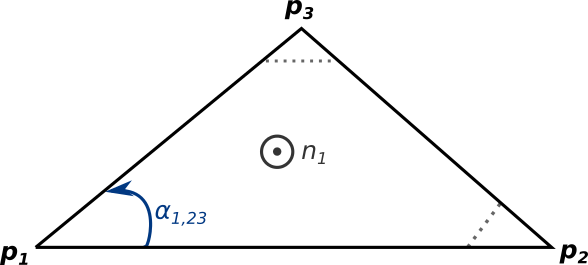
\includegraphics[width=.6\linewidth]{assets/3-face_force_face.png}
\end{figure}

As previously, face constraints are modeled as a linear-elastic spring.
For each of the interior angle of a triangular face, forces are applied to its neighbouring vertices.

\begin{equation} \label{solver:face_force}
	\pmb{F}_{face} = -k_{face}(\alpha - \alpha _0)\frac{\partial \alpha}{\partial \pmb{p}}
\end{equation}

where

\begin{itemize}
	\item $k_{face}$ is a face stiffness
	\item $\alpha$ is a current interior angle
	\item $\alpha _0$ is an initial interior angle
\end{itemize}

Derivatives of $\alpha$ with respect to $p$ are given by

\begin{equation} \label{solver:face_force1}
	\frac{\partial \alpha _{2,31}}{\partial \pmb{p}_1} = \frac{\pmb{n} \times (\pmb{p}_1 - \pmb{p}_2)}{\norm{\pmb{p}_1 - \pmb{p}_2}^2}
\end{equation}

\begin{equation} \label{solver:face_force2}
	\frac{\partial \alpha _{2,31}}{\partial \pmb{p}_2} = \frac{\pmb{n} \times (\pmb{p}_1 - \pmb{p}_2)}{\norm{\pmb{p}_1 - \pmb{p}_2}^2} + \frac{\pmb{n} \times (\pmb{p}_3 - \pmb{p}_2)}{\norm{\pmb{p}_3 - \pmb{p}_2}^2}
\end{equation}

\begin{equation} \label{solver:face_force3}
	\frac{\partial \alpha _{2,31}}{\partial \pmb{p}_3} = \frac{\pmb{n} \times (\pmb{p}_3 - \pmb{p}_2)}{\norm{\pmb{p}_3 - \pmb{p}_2}^2}
\end{equation}


\medskip
\textbf{Damping - damping force}
\smallskip

Damping is an additional force that is not required from the modeling perspective,
but is required from the solver's stability point of view. It prevents model's
oscillation while folding and without it barely any model folds correctly.

\begin{figure}[H]
	\caption{Damping force formulation on the two vertices connected by an edge}
    \centering
	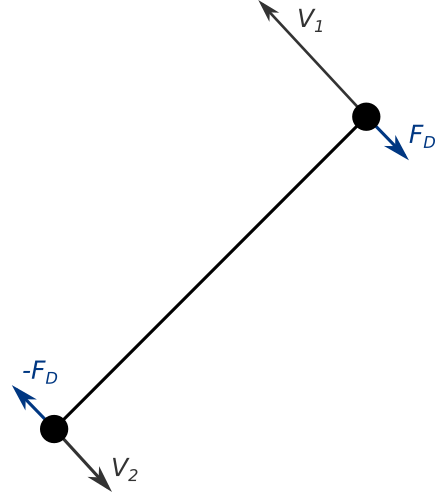
\includegraphics[width=.4\linewidth]{assets/3-damping_force_edge.png}
\end{figure}

Damping force is defined in terms of vertices' velocity as:


$$F_{damping} = -e_{damping} * (V_1 - V_2)$$

where:

\begin{itemize}
	\item $e_{damping}$ is a damping coefficient 
	\item $V_1$ and $V_2$ are vertices' velocities
\end{itemize}

For each edge damping coefficient is set as:

$$ e_{damping} = d_p * 2 * \sqrt{k_{axial} * min(v1_{mass}, v2_{mass})} $$

where:

\begin{itemize}
	\item $d_p$ is a configurable damping percent
	\item $k_{axial}$ is axial stiffness defined previously
	\item $vx_{mass}$ is mass of a vertex $x$
\end{itemize}

We assume that mass is constant for each vertex.

As is the case for beam force, damping force is computed in a model's coordinate space
and then applied to each of the edge's vertices.
\smallskip

\begin{figure}[H]
	\centering
	\caption{The code carrying out damping force calculation}
	\lstinputlisting{assets/listings/damping_force.py}
\end{figure}

\medskip
\textbf{Numerical integration}
\smallskip

Once all the forces are defined, the total force for each vertex is computed as a sum of all the imposed forces.

\begin{equation} \label{solver:total_force}
	\pmb{F}_{total} = \sum_{edges} \pmb{F}_{beam} + \sum_{edges} \pmb{F}_{crease} + \sum_{faces}\pmb{F}_{face} + \sum_{edges}\pmb{F}_{damping}
\end{equation}

Then using Newton's Second Law of Dynamics we compute acceleration as:

$$
\pmb{a} = \frac{\pmb{F}_{total}}{m}
$$

where $m$ is a vertex's mass. We assumed that mass is constant for each vertex, however a more appropriate analysis could yield
better results in terms of folding dynamics.

Having acceleration, we compute vertex velocity and next position using \textit{forward Euler Integration} method:

$$
\begin{aligned}
\pmb{V}_{t+\Delta t} = \pmb{V}_t + \pmb{a}\Delta t \\
\pmb{p}_{t+\Delta t} = \pmb{p}_t + \pmb{V}\Delta t
\end{aligned}
$$

We assume the initial conditions:

\begin{equation}
	\begin{aligned}
		\pmb{V}_0 = 0\\
		\pmb{p}_0 = \text{provided by Instruction}
	\end{aligned}
\end{equation}


As an end condition we check whether the difference between current and previous forces is smaller than some configured $\varepsilon$:

\begin{lstlisting}[language=Python]
diff = np.abs(np.array(current_forces) - np.array(previous_forces))
return np.all(diff <= epsilon)
\end{lstlisting}

To generate all the Transitions in the model we run the solve function for each step in the Instruction.

\begin{figure}[H]
	\caption{The simplified pseudocode for the solving process}
	\lstinputlisting{assets/listings/solver.py}
\end{figure}


\subsection{Quality assurance}

To ensure the quality of the application, the codebase is continuously linted, tested, built, and delivered. Immediate feedback is available for developers, code reviewers, and operators, reducing the possibility of merging a faulty code into the \texttt{master} branch and therefore using a faulty deployment in the production environment.

\medskip
The pipeline is implemented using \tech{Github Actions}, which is a part of \tech{Github}. This allows for seamless integration with the code repository.

\medskip
Furthermore, no changes can be pushed directly to the \texttt{master} branch. Every commit needs to be reviewed by at least one other developer before being merged. This policy is enforced using \tech{Github} settings.

\medskip
Each system component has a dedicated pipeline, tailored to specific requirements. 

\medskip
Continuous delivery and deployment negate the risk of deploying an application that has not passed all the required checks in the pipelines.

\medskip
All of the dependencies are bound to a specific minor version. Doing so ensures that in case one of the vendors implements a breaking change our application and pipelines will not break.

\subsubsection{Frontend}

The frontend code is linted on every commit using \tech{Husky}, \tech{ESLint}, and \tech{Prettier}. It is not possible to push an incorrectly formatted code to the repository.
Uniformly formatted code improves the clarity, allowing a code reviewer to focus on business logic and potential bugs instead of code-formatting.

\medskip

To aid the code review process every pull request containing changes related to the frontend component is deployed as a \tech{preview application} on \tech{Netlify}. A \tech{preview application} is an isolated environment with an application built using the code submitted along with a pull request.

\medskip

Most of the business logic on the frontend is tested. The test runner of choice is \tech{Jest}. Running the whole test suite is as simple as executing \texttt{yarn test}.

\begin{figure}[H]
  \caption{Workflow - frontend component. Every commit is tested and built.}
  \centering
    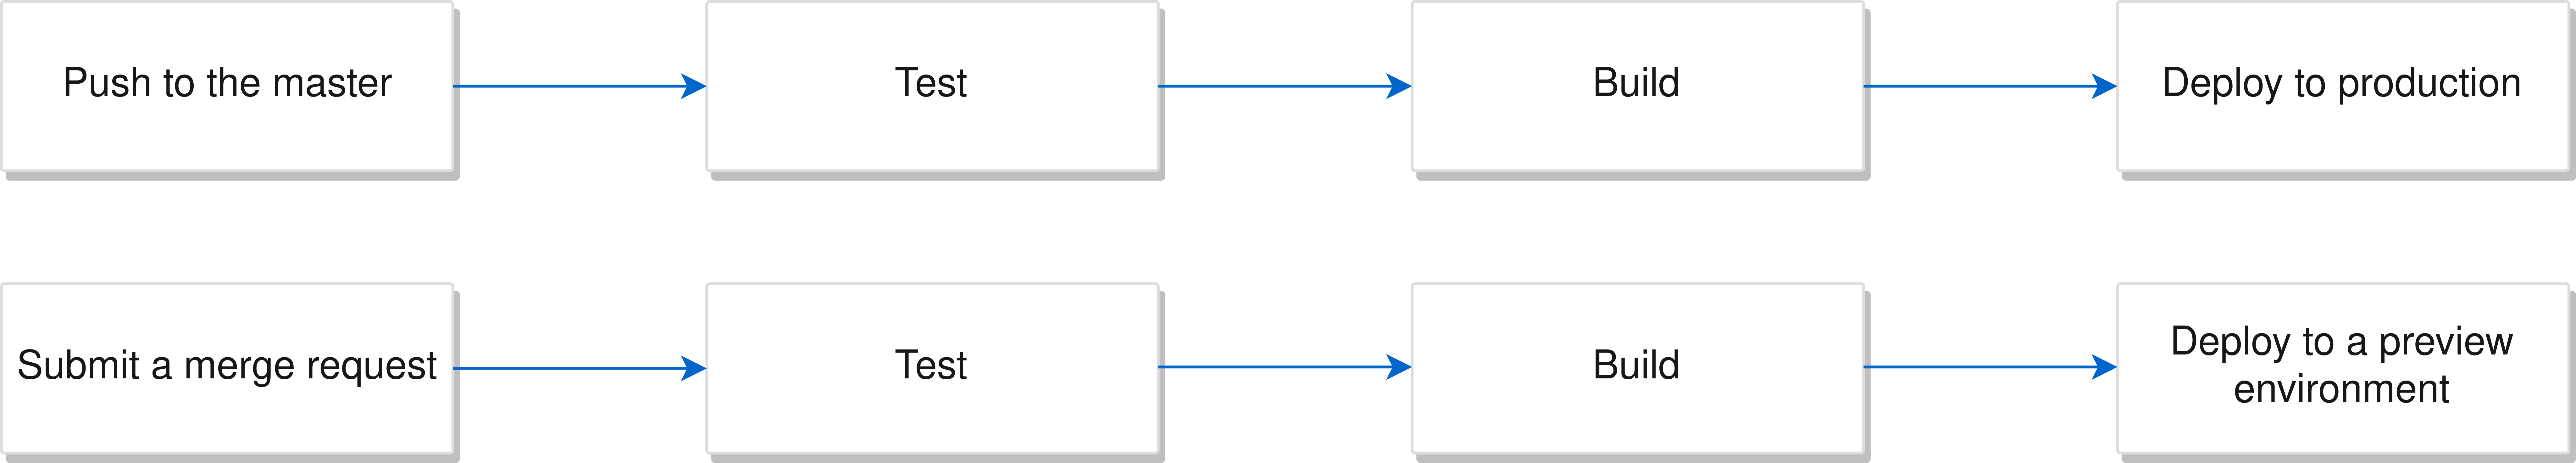
\includegraphics[width=\textwidth]{assets/3-frontend-pipeline.png}
\end{figure}

\subsubsection{Solver}

Solver is a library written in \tech{Python} and tested using the \tech{unittest} module. Most of the business logic is covered. 

The line test coverage is 77\%.

\begin{figure}[H]
  \caption{Workflow - solver component. Every change is tested.}
  \centering
    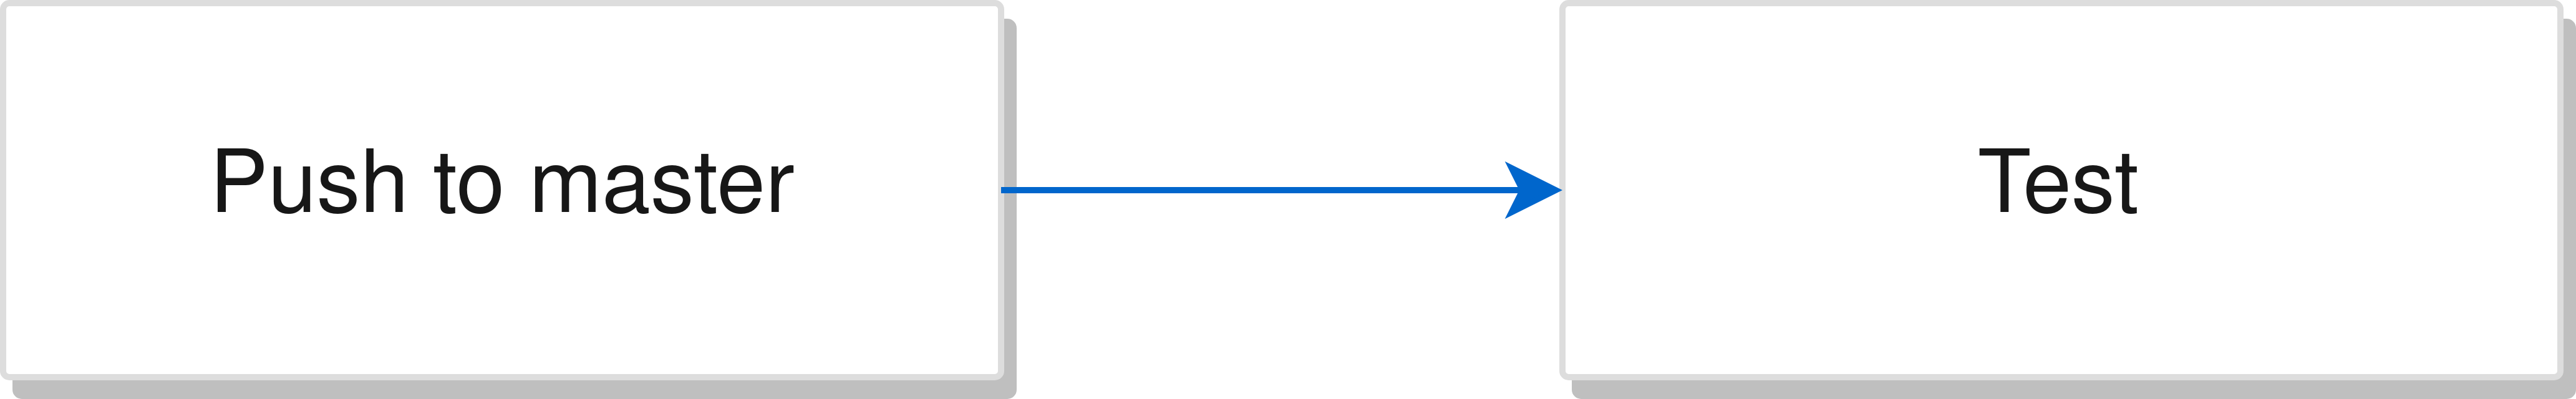
\includegraphics[width=0.8\textwidth]{assets/3-solver-pipeline.png}
\end{figure}


\subsubsection{Community}

The Community backend is written in \tech{Python} using \tech{Django} and therefore uses the \tech{unittest} module that is built-in to the Python standard library. All of the public-facing endpoints are fully covered with integration tests verifying that authentication, authorization, and request body handling are properly implemented. The line test coverage is 96\%.

\medskip
Code style abides by the \tech{PEP8} standard.

\medskip
To ensure build reproducibility, the Community backend is enclosed in a Docker image that is automatically deployed to a production environment. 

\begin{figure}[H]
  \caption{Pipeline - Community backend.}
  \centering
    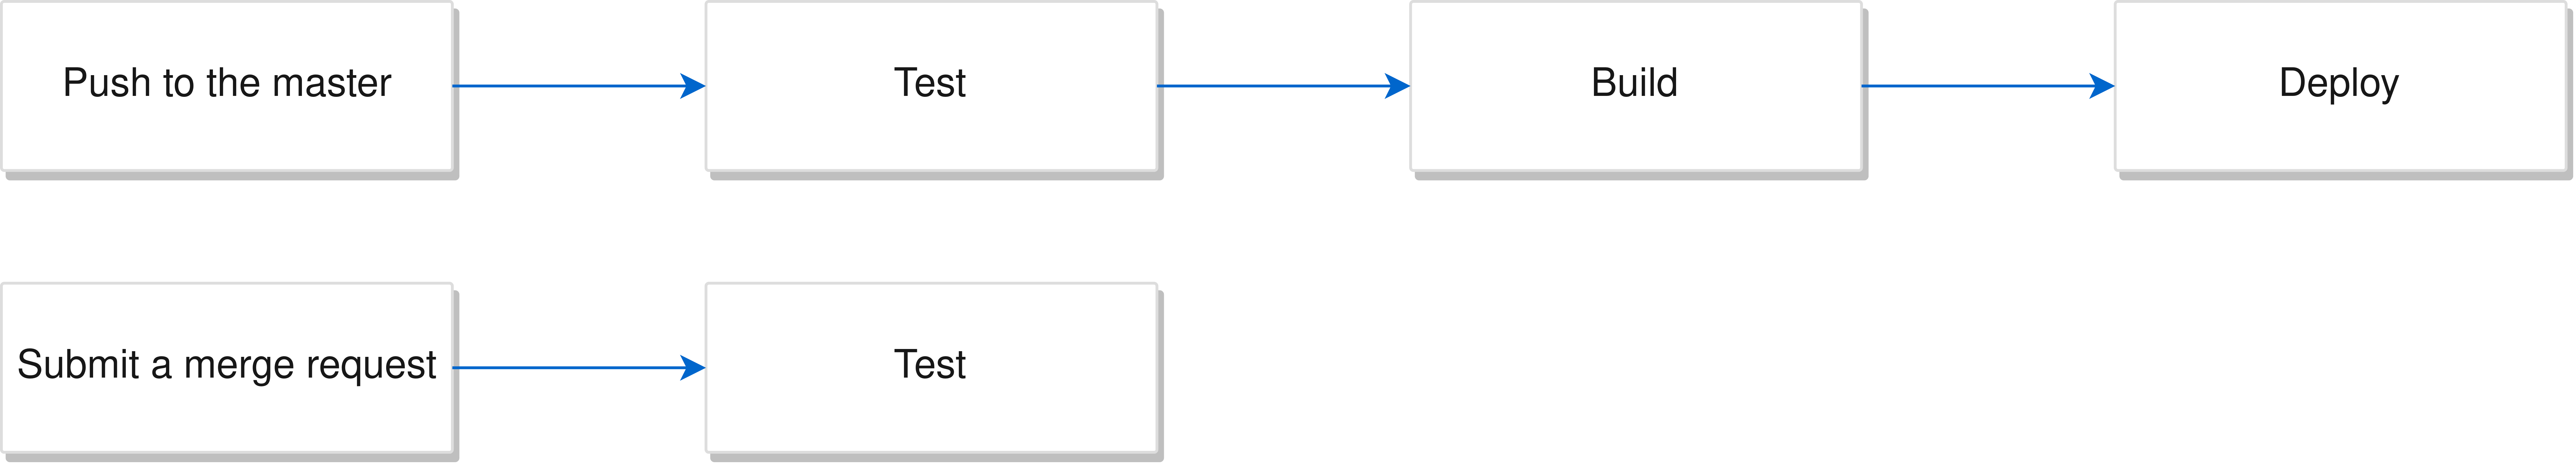
\includegraphics[width=\textwidth]{assets/3-community-pipeline.png}
\end{figure}

\subsection{Deployment}

Origuide uses \tech{Docker} images for packaging backend components. Images are pushed to the \tech{Docker Hub} repository where they are publicly available. The frontend build output consists of a set of static files.

\medskip
The backend deployment configuration is specified using \tech{docker-compose} files. 
Because all the environment specific configuration is externalized to \texttt{.env} files, the deployment configuration remains environment agnostic. This makes Origuide's backend deployable using a single command.

\begin{figure}[H]
	\caption{Example configuration of an \textit{.env} file}
	\lstinputlisting{assets/listings/3-8-env-file}
\end{figure}

\begin{figure}[H]
	\caption{An example of a command that deploys the backend components.}
	\begin{lstlisting}
docker-compose up -d
	\end{lstlisting}
\end{figure}

The frontend component can be easily deployed to any file hosting solution using a file transfer with no additional configuration requirement. This configuration-less nature of the deployment allows switching hosting providers easily should a need arise.

\begin{figure}[H]
	\caption{An example of a command that deploys the frontend components.}
	\begin{lstlisting}
scp -r ./dist user@{hosting-provider}:/www 
	\end{lstlisting}
\end{figure}
\medskip

\textbf{Production environment}

The backend production environment is running on servers provided by \tech{Digital Ocean}.

\medskip
The frontend is built and deployed on \tech{Netlify}.




% Instrukcja postawienia środowiska deweloperskiego - jeśli potrzeba wypełniacza %


\subsection{Problems encountered}
% Z jakimi problemami technicznymi sie borykaliście? Jeśli nie opisaliście ich w dokumentacji procesowej. %
% Collissions
\subsubsection{Collision detection and handling}
\subsubsection{Damping force}
\subsubsection{Paper stiffness}
\subsubsection{Unnatural guide encoding}

\subsubsection{Mesh rendering hazard}

When folding origami models, two faces lying flat on each other are a common occurrence.

The Solving algorithm is not sophisticated enough to have a sense of sheet thickness. Therefore, it places the folded faces close to each other, on the verge of numerical error. The rendering engine cannot distinguish which face is on top and which one is below, resulting in a face color mixture demonstrated below.

\begin{figure}[H]
	\caption{An example of a mesh rendering hazard}
  \centering
    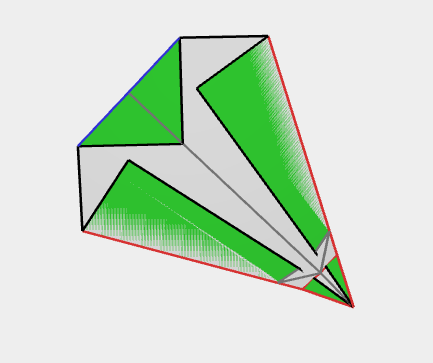
\includegraphics[width=0.6\textwidth]{assets/3-rendering-hazard.png}
\end{figure}

Unfortunately, the issue has not been resolved in the current iteration. Some potential solutions include:
\begin{itemize}
	\item preventing faces from colliding during solving,
	\item detecting interpenetrating faces after solving and marking which one is on top.
\end{itemize}

\subsubsection{Large web application bundle size}

The frontend application uses multiple feature-rich libraries of significant file size footprint such as \tech{Three.js} or \tech{Material-UI}. The whole bundle size was $ 6.81\mathrm{MB} $ resulting in a non-ideal download and parsing times of several seconds.

\medskip
To analyze the size of all bundle components, \tech{BundleAnalyzerPlugin} for \tech{Webpack} was used. 

\medskip

\begin{figure}[H]
	\caption{The output of the analysis is in the form of an interactive website that allows drilling down and identifying potential areas of improvement.}
  \centering
    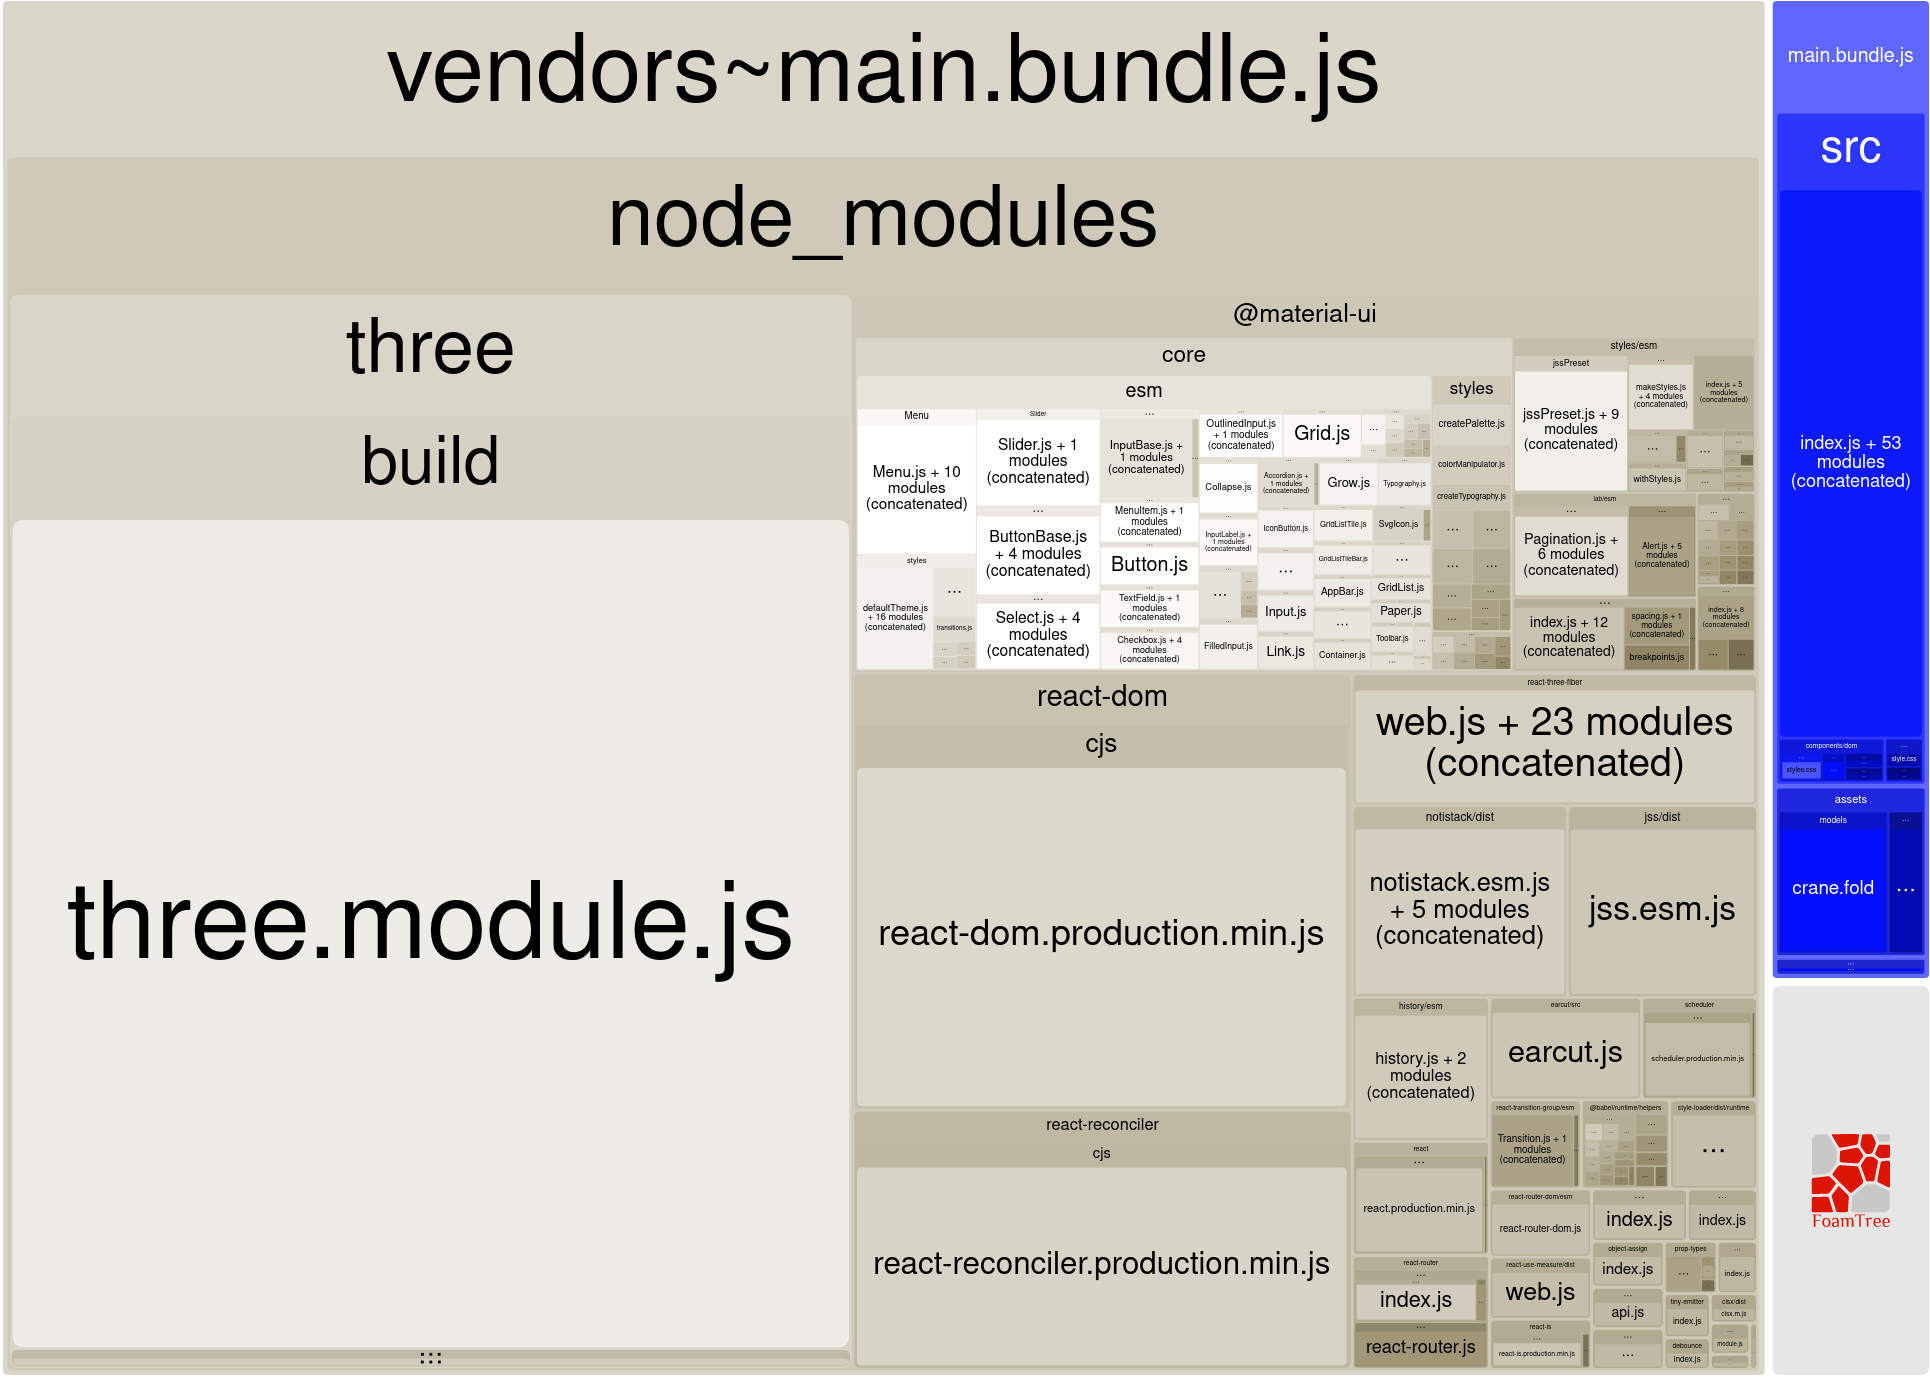
\includegraphics[width=\textwidth]{assets/3-bundle.png}
\end{figure}

To optimize the application size several techniques have been used:

\begin{description}
	\item[tree-shaking] - dead code elimination technique
	\item[minimizing] - unnecessary character removal
	\item[chunking] - code splitting and on-demand chunk loading
\end{description}

The minimizing was done using the \tech{Terser} plugin. Chunk splitting and tree-shaking features are included, but not enabled by default, in \tech{Webpack}.

\begin{table}[H]
\label{bundle-size-optimizations}
\caption{Incorporating optimizations reduced the bundle size massively, cutting the load time by a large factor.}
\begin{minipage}[t]{\linewidth}
\begin{tabular}{|l|l|l|l|l|}
\hline
\multicolumn{1}{|c|}{} & \multicolumn{2}{l|}{Before optimizations} & \multicolumn{2}{l|}{After optimizations} \\ \hline
                       & Size                & Gzipped            & Size                & Gzipped            \\ \hline
Three.js               & 1.2MB               & 233.82KB           & 624.87KB            & 148.83KB           \\ \hline
Material-UI            & 701.28KB            & 122.62KB           & 196.81KB            & 56.33KB            \\ \hline
Application size       & 6.81MB              & 1.52MB             & 1.2MB               & 322.15KB           \\ \hline
\multicolumn{1}{|l|}{Load time\footnotemark} & \multicolumn{2}{c|}{4.24s} & \multicolumn{2}{c|}{0.81s} \\ \hline
\end{tabular}
\footnotetext{Duration calculated between client-connection connection establishment and \texttt{load} DOM event being fired}
\end{minipage}
\end{table}

\subsubsection{Generating thumbnails for computed Guides}

As of now, Guide thumbnails represent a flat crease pattern. Ideally, the Guide's image would contain a fully folded model. The functionality is not trivial to implement and, due to other issues having a higher priority, has not been worked on.

\begin{figure}[H]
	\caption{A guide thumbnail with a crease pattern}
  \centering
    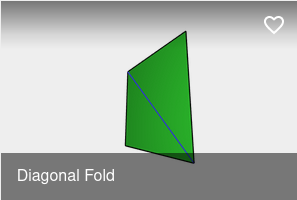
\includegraphics[width=0.3\textwidth]{assets/3-thumbnails.png}
\end{figure}

\medskip


A couple of potential implementations include:

\begin{itemize}
	\item Capturing a generated model on the first model view (that is how a crease pattern preview is currently implemented).
	\item Spinning up a headless browser instance, loading a model, and making a screenshot.
	\item Rendering a final solver step on the Solver backend using a plotting library.
\end{itemize}


